% LaTeX Vorlage für studentische Arbeiten am imes, MZH, ...
% Vorlagenversion vom 15.08.2017
%
%
%
%
%
% META & VOREINSTELLUNGEN -------------------------------------------------------
\newcommand{\Autor}%                % Name des Autors / der Autorin
{Andreas Serov}
\newcommand{\Matrikelnummer}%       % Matrikelnummer
{2871560}
\newcommand{\Datum}%       				 % Abgabedatum
{30. September 2018}

% ------------------------------------------------------------------------------------------
% erlaubt das Anfangen des Draft-Modus und damit Veränderungen
% einzustellen
\newif\ifdraft
% Draft-Modus: Arbeitsversion, Bilder werden nur als Rahmen dargestellt
% Vorteil: schnelleres Kompilieren
%\drafttrue % <- dafür hier die Kommentierung wegnehmen

%-------------------------------------------------------------------------------------------
% folgende Befehle sorgen dafür, das für jede Schrift die richtigen Pakete installiert werden
\newcounter{schrift}
% Schrift auswählen:
% 1 - mathptmx
% 2 - minionpro
% 3 - mathpazo
% 4 - times + computer modern
% 5 - computer modern
\setcounter{schrift}{4} % Hier die entsprechende Zahl setzen !

% ------------------------------------------------------------------------------------------
% ------------------------------------------------------------------------------------------
% Latex - Präambel
% hier werden alle wichtigen Dokumenteinstellungen getroffen, normalerweise müssen
% keine Änderungen mehr durchgeführt werden.
% Pakete die das Schriftbild, den Satzspiegel oder die Ränder verändern, dürfen
% nicht hinzugefügt werden, erst nach Abstimmung mit dem Betreuer.
% nützliche Pakete sind willkommen, bitte die Wiki entsprechend aktualisieren
% viele Pakete sind drin, die vielleicht nicht jeder braucht und das Kompilieren verlängern
% sollten diese das Layout nicht verändern, können diese natürlich auskommentiert werden.
% ------------------------------------------------------------------------------------------

% ------------------------------------------------------------------------------------------
% Dokumentenklasse definieren:
\ifdraft
    \documentclass[draft, 
                   paper=a4,
                   BCOR5mm,
                   fontsize=12pt, 
                   DIV13, 
                   headsepline, 
                   numbers=noenddot, 
                   %bibtotoc,
                   bibliography = totoc,
                   %version=first,
                   %smallheadings,
                   headings = small,
                   oneside]{scrbook}
\else
    \documentclass[paper=a4,
                   BCOR5mm,
                   fontsize=12pt, 
                   DIV13, 
                   headsepline, 
                   numbers=noenddot, 
                   %bibtotoc,
                   bibliography = totoc, 
                   %version=first,
                   %smallheadings,
                   headings = small,
                   headinclude=true,
                   footinclude=false,
                   %fleqn, % formeln links bündig
                   oneside]{scrbook}
\fi
% Standard-Koma-Dokument mit
%   Papierformat A4
%   Binderand 5 mm
%   Schrift 12-Punkt
%   Seitenlayout nach DIV, siehe scrguide.pdf text b/h rand oben/innen: 168,00 237,60 19,80 14,00 (ist raus)
%   Linie unter der Kopfzeile
%   Nummern ohne Punkt am Ende
%   Literaturverzeichnis im Inhaltsverzeichnis
%   Überschriften etwas kleiner als standard
%   weitere Informationen zum Koma-Skript: www.komascript.de

%---------------------------------------------------------------
% Basis-Pakete
%---------------------------------------------------------------
\usepackage{ifpdf}		%   Ueberprueft, ob LaTeX oder pdfLaTeX verwendet wird (nur ab MikTeX 2.5)
\usepackage[T1]{fontenc}        %   8-Bit-Fonts
\usepackage{textcomp,latexsym}  %   zusaetzliche Symbole
\usepackage[utf8]{inputenc}   %   Quelltext ist Latin-1 (d.h. Windows-) kodiert
\usepackage[ngerman]{babel}            %   neue deutsche Rechtschreibung
\usepackage{scrtime}            %   fuer die aktuelle Zeit
%\usepackage{scrdate}            %   fuer das aktuelle Datum
%\usepackage{natbib}             %   Literaturverweise mit (Autor Jahr) nach DIN
%\bibpunct[; ]{[}{]}{,}{a}{}{;}  %   eckige Klammern statt runde bei Zitaten
%\usepackage[T1]{url}            %   Web-Addressen auch mit T1-Encoding
%\urlstyle{tt}                   %   und in tt-Font
%\usepackage[activate=normal]{pdfcprot} % dient dem optischen Randausgleich bei kürzeren Zeichen wie '-', '.', ',', '!'

\usepackage{color}



\PassOptionsToPackage{x11names}{xcolor}
\usepackage{xcolor}


%---------------------------------------------------------------
% nützliche Zusatz-Pakete
%---------------------------------------------------------------
%\usepackage{makeidx}            %   Index (wenn gewuenscht)

\usepackage{setspace}           %   Zeilenabstand setzen. Befehl:
                                %   \begin{spacing{Wert}
                                %   Text
                                %   \end{spacing}
%\usepackage{placeins}           %   das Positionieren von float-Umgebungen bestimmen:
                                %   der Befehl \floatbarrier sorgt dafür, dass alle vorher eingegebenen
                                %   float-Umgebungen VOR diesem Befehl eingefügt werden.
                                
%\usepackage{subfig}          %   Bilder gruppieren, mehrere Bilder in einer Umgebung einfügen
                                %   Bsp.:
                                %   \begin{figure}
                                %   \centering
                                %    \subfloat[Text a]
                                %    {\includegraphics{bild a}}
                                %    \subfloat[text b]
                                %    {\includegraphics{bild b}}
                                %    \caption{Untertitel}
                                %    \label{fig.Beziechnung_subfigure} <- am besten mit fig. dann kann mit \bild{Bezeichnung_figure} referenziert werden
                                %   \end{figure}                                

%\usepackage{textcomp}           %   fuer Trademark und Copyright Zeichen
                                %   z.B \texttrademark, \textregistered, \texteuro etc.

\usepackage{tabularx}           %   erweiterte Funktionen für Tabellen

\usepackage{longtable}          %   Longtable-Package für Tabellen die länger als eine DIN-A4-Seite sind

\usepackage{colortbl}						%		farbige Tabellenzeilen

\usepackage{nicefrac}           %   Schräge Bruchstriche \nicefrac{Nenner}{Zähler}

%\usepackage{numprint}           %   Zahlen mit Einheiten näher an der Zahl/kein Umbruch und 1 000er Format \numprint[Einheit]{Zahl}

%\usepackage{mathcomp}           %   für \tcdegree (° Gradzeichen bei numprint) \numprint[\tcdegree]{180} für 180°

%\usepackage{hhline}             %   hhline-Package
                                %   Fuer komplexe Linienzuege in Tabellen \hhline{}
                                %   = Spalte mit doppelter Linie      | vertikale Linie die horizontale schneidet
                                %   - Spalte mit einfacher Linie      : vertikale Linie die von horizantaler unterbrochen ist
                                %   ~ Spalte ohne Linie               # doppelte horiz. geschnitten mit doppelter vert. Linie
                                %   t oberer Teil ->                  b unterer Teil einer doppelten Linie

%\usepackage[active]{srcltx}     %   bei verwendung v. \includeonly spring winedt jetzt bei fehlern an die richtige stelle

\usepackage{flafter}            %   Ein float-Objekt immer erst NACH seiner Definition platzieren

\usepackage{ifthen}             %   definiert \ifthenelse{}{}{}

%\usepackage{path}               %   dateinamen und pfade darstellen

%\usepackage{pdfsync}						%   Synchronisation mit SumatraPDF <<-- geht auch ohne

\usepackage{booktabs}

\usepackage{scrhack} % Löscht Warnungen von Packages wie hyperref, listings
\usepackage[ locale = DE,            % deutsch
            load-configurations=abbreviations, % zusätzliche Einheiten siehe manual
            per-mode=symbol,%-or-fraction,
            separate-uncertainty% 
            ]
            {siunitx}								% SI-Einheiten  
						\sisetup{detect-all} % aktuelle Schriftart nutzen (statt immer Mathemodus)

            
\usepackage{multirow}               % zwei Zeilen kombinieren (wie multicolumn)
\usepackage[babel]{microtype}       % schickeres Schriftbild -> aber längeres Kompilieren

\usepackage{blindtext}							% sinnlosen text einbauen
%\usepackage{subfigure}

\usepackage{newunicodechar}
%\newunicodechar{ }{~}


%---------------------------------------------------------------
% Andreas Serov hinzugefügte Pakete
%---------------------------------------------------------------
\usepackage{bm}					% bold math symbols
\usepackage{tikz}				% graphics via tikz

% custom colors
\definecolor{imesblue}{rgb}{0.00000,0.313725,0.607843}			
\definecolor{imesorange}{rgb}{0.90588235,0.48235,0.160784}
\definecolor{imesgreen}{rgb}{0.784313,0.82745,0.090196}%
%% tikz libraries und styles, die allgemein für Grafiken verwendet werden
\usetikzlibrary{shapes,arrows, positioning}
% kreis, rechteck und pfeil mit in imesblau
\tikzstyle{simplecircle} = [draw, circle, node distance=2.5cm, line width=3pt, color=imesblue]
\tikzstyle{simplebox} = [draw, rectangle, node distance=2.5cm, line width=3pt, color=imesblue, rounded corners]
\tikzstyle{simplearrow} = [draw, -latex, line width=2pt, color=imesblue]

\usepackage{lipsum} 			% zum Einfügen von Paragraphen von text
\usepackage{wrapfig}			% Bild und Textfluss, gibt wohl bessere Alternativen

\usepackage{subcaption}		% für subfigures, package "subfigure" deprecated

\usepackage{gensymb}

%\DeclareUnicodeCharacter{00A0}{~}

%---------------------------------------------------------------
% Grafik-Paket für eps bzw. pdf
%---------------------------------------------------------------
% überprüft ob Latex oder PDFLatex ausgeführt wird, dementsprechend werden pdf/jpg oder eps Bilder eingefügt
% sollen dvi oder pdf Dokumente erstellt werden müssen alle Bilder in beiden Formaten vorliegen
% hierfür gibt es Tools wie epstopdf oder jpgtoeps
 \ifdraft
    \usepackage[draft]{graphicx}
\else
    \ifpdf
        \usepackage{graphicx}
        \usepackage{pgfplots} % pgfplots zum plotten in LaTeX
    \else
        \usepackage[final]{graphicx}
    \fi
\fi
% von wo sollen die Grafiken kommen?

\graphicspath{{./bilder/}{./bilder/kinematik/}{./bilder/standdertechnik/}}

%\graphicspath{{./bilder/titel}}
%\graphicspath{{./bilder/einleitung}}
%\graphicspath{{./bilder/standdertechnik}}
%\graphicspath{{./bilder/kap3}}
%\graphicspath{{./bilder/kap4}}


%Einstellungen für pgfplots
\pgfplotsset{compat=1.3,
	%enlargelimits=auto,
	tick label style={font=\small,/pgf/number format/use comma}, %Komma nutzen in allen Axen
	%axis x line=center, %alle x-Achsen center
	%axis y line=center, %alle y-achsen center
	%every axis x label/.style={at={(current axis.right of origin)},anchor=west}, % achsenbeschriftung bei allen x-achsen rechts
	%every axis y label/.style={at={(current axis.above origin)},anchor=south},   % achsenbeschriftung bei allen y-achsen oben
	%every x tick scale label/.style={at={(current axis.right of origin)},anchor=north,yshift=-0.5em}, %positionierung des scale faktors geändert
	every axis legend/.append style={at={(0.5,1.03)},anchor=south,nodes=right,font=\small}, % Legende über der Grafik, schriftgröße small
	label style={font=\small} % label schriftgröße small
}
\newlength\tikzwidth
\setlength{\tikzwidth}{0.7\textwidth}
\definecolor{mycolor1}{rgb}{0,0.5,0}

\ifpdf
 \ifdraft
    \usepackage[draft]{pdfpages}%   externe PDF Seiten einbinden nur bei PDF-Latex möglich
    \else
    \usepackage[final]{pdfpages}%   externe PDF Seiten einbinden nur bei PDF-Latex möglich
 \fi                            %   Befehl: \includepdf{PDF-Datei} soll die Datei im Querformat angezeigt werden
    \else
\fi                             %   \includepdf[landscape=true]{PDF-Datei}

%---------------------------------------------------------------
% Debug-Ausgabe der Labels und References
%---------------------------------------------------------------
\ifdraft
  \usepackage{showkeys} % Label werden im Draft Modus im Text angezeigt
\fi

%---------------------------------------------------------------
% Abweichende PostScript-Schriftarten
% werden in der main Datei ausgewählt, hier nichts ändern
%---------------------------------------------------------------
\ifthenelse{\equal{ 1 }{ \value{schrift} }}
    {
    \usepackage{mathptmx}          %   Times als Hauptschriftart, keine mathematische Fettschrift
    \usepackage{amssymb}
    \usepackage{amsbsy}
    \usepackage{amsmath}
    \usepackage{amsfonts}
    \usepackage{amstext}
    \renewcommand{\boldsymbol}[1]{\mathbf{#1}} % nur bei mathptmx !
                                               % damit boldsymbol wenigstens fette aufrechte Buchstaben macht
    }{}
\ifthenelse{\equal{ 2 }{ \value{schrift} }}
    {
    \usepackage[lf, minionint]{MinionPro} %   OpenType von Adobe, mathematische Fettschrift vorhanden, Schrift ist
                                %   ist im Standard-LaTeX nicht installiert.
                                %   Ist ein wenig Aufwand das Ganze zu installieren, Matthias Dagen fragen
    }{}
\ifthenelse{\equal{ 3 }{ \value{schrift} }}
    {
    \usepackage{mathpazo}          %   nette Buchschrift aber sehr gross, mathematische Fettschrift vorhanden
    \usepackage{amssymb}
    \usepackage{amsbsy}
    \usepackage{amsmath}
    \usepackage{amsfonts}
    \usepackage{amstext}
    }{}
\ifthenelse{\equal{ 4 }{ \value{schrift} }}
    {
    \usepackage{times}
    \usepackage{amssymb}
    \usepackage{amsbsy}
    \usepackage{amsmath}
    \usepackage{amsfonts}
    \usepackage{amstext}
    }{}
\ifthenelse{\equal{ 5 }{ \value{schrift} }}
    {
    \usepackage{amssymb}
    \usepackage{amsbsy}
    \usepackage{amsmath}
    \usepackage{amsfonts}
    \usepackage{amstext}
    \usepackage{lmodern}
    }{}
\usepackage[scaled=.92]{helvet} %   11pt Helvetica für Überschriften etc. etwas kleiner da, Helvetica an sich größer ist
%\usepackage{courier}            %   Courier bei \texttt
%\usepackage{upgreek}            %   Aufrechte griechische Buchstaben

% ------------------------------------------------------------------------------------------
% Bild- und Tabellentitel FETT
% ------------------------------------------------------------------------------------------
%\def\figurename{\bfseries Bild}
%\def\tablename{\bfseries Tabelle}

%%Andere Beschreibung von figure
\addto\captionsngerman{
	\renewcommand{\figurename}{\bfseries Bild}%%Andere Beschreibung von figure
	\renewcommand{\listfigurename}{Bildverzeichnis}
	\renewcommand{\tablename}{\bfseries Tabelle}
}

%---------------------------------------------------------------
% Quelltexte formatieren
%---------------------------------------------------------------
\usepackage{listings}


%\lstloadlanguages{
		%C,
		%C++,
		%XML
%}

\lstset{
		language=XML,
		basicstyle=\footnotesize\ttfamily, % Standardschrift
		numbers=left,               % Ort der Zeilennummern
		numberstyle=\tiny,          % Stil der Zeilennummern
		numbersep=5pt,              % Abstand der Nummern zum Text
		tabsize=2,                  % Groesse von Tabs
		extendedchars=true,         %
		breaklines=true,            % Zeilen werden Umgebrochen        
		keywordstyle=\color{Red2},
		frame= b,         
		stringstyle=\color{Purple2}\ttfamily, % Farbe der String
		showspaces=false,           % Leerzeichen anzeigen ?
		showtabs=false,             % Tabs anzeigen ?
		xleftmargin=17.5pt,
		framexleftmargin=17pt,
		framexrightmargin=5pt,
		framexbottommargin=4pt,
		linewidth= \dimexpr\textwidth-2\fboxsep-2\fboxrule,
		comment=[l]{\#},
		morecomment=[s]{<!--}{-->},
		commentstyle=\color{Green4},
		%backgroundcolor=\color{grey},
		showstringspaces=false,      % Leerzeichen in Strings anzeigen ?        
		morekeywords={__global__, name, pkg, args, type, from, to, textfile, respawn, value, output, radius, ixx, ixy, ixz, iyy, iyz, xyz, rpy, reference},  % CUDA specific keywords
		aboveskip = 18pt, 
		belowskip = 18pt
}

\usepackage{caption}
\DeclareCaptionFont{white}{\color{white}}
\DeclareCaptionFormat{listing}{\colorbox{darkgray}{\parbox{\dimexpr\textwidth-2\fboxsep-2\fboxrule}{\hspace{15pt}#1#2#3}}}
\captionsetup[lstlisting]{format=listing,labelfont=white,textfont=white, singlelinecheck=false, margin=0pt, font={bf,footnotesize}}

%---------------------------------------------------------------
% ein paar Längen einstellen
%---------------------------------------------------------------
%\setlength{\parskip}{1ex plus0.5ex minus0.2ex} % Absatzabstand etwas größer
\setlength{\itemsep}{0ex plus0.2ex}            % Abstand zweier Listenelemente kleiner
\setlength{\parindent}{0ex}                     % kein Absatzeinzug
\setlength{\belowcaptionskip}{0.4cm}            % Abstand caption - Tabelle größer
\setlength{\abovecaptionskip}{0.4cm}            % Abstand caption - Tabelle größer

%---------------------------------------------------------------
% Kopf- und Fusszeilen
%---------------------------------------------------------------
\usepackage[plainheadsepline,  % linie zw. kopf und text auch bei seitenstil "plain"
           %headexclude,       % kopfzeile gehört nicht zum textkörper
           %footexclude        % fusszeile gehört nicht zum textkörper
          ]       
           {scrpage2}
\pagestyle{scrheadings}
\clearscrheadfoot              % voreinstellungen loeschen
\ihead{\normalfont\headmark}   % kolumnentitel innen
\ohead[\pagemark]{\pagemark}   % seitenzahl aussen

%---------------------------------------------------------------
% Nummerierungs-Tiefe des Inhaltsverzeichnis und der Abschnitte einstellen
%---------------------------------------------------------------
\setcounter{secnumdepth}{2} \setcounter{tocdepth}{2}

%---------------------------------------------------------------
% Abkürzungsverzeichnis
%---------------------------------------------------------------
% mit dem Befehl \nomenclature[l/g/a]{Abkürzung}{Bezeichnung} kann direkt im Code die Abkürzung eingefügt werden
% das Paket sortiert diese und fügt sie mit dem Befehl \printnomenclature ein
% l, g, oder a steht dabei für die Gruppierung Lateinische bzw. Griechische Buchstaben, Abkürzungen
% Nach Einfügen neuer Abkürzungen muss folgender Befehl in der Eingabeaufforderung im Tex-Verzeichnis eingegeben werden:
% -> vorher einmal kompilieren
% -> makeindex main.nlo -s nomencl.ist -o main.nls
% -> nochmal kompilieren
%\makeindex
\usepackage{nomencl}
% \let\abbrev\nomenclature
\renewcommand{\nomname}{Abkürzungsverzeichnis}
\setlength{\nomlabelwidth}{.25\hsize}
\renewcommand{\nomlabel}[1]{#1 \hfill}
\setlength{\nomitemsep}{-\parsep}

\renewcommand{\nomgroup}[1]{%
	\ifthenelse{\equal{#1}{L}}{\item[\textbf{Lateinische Buchstaben}]}
	{%
		\ifthenelse{\equal{#1}{G}}{\item[\textbf{Griechische Buchstaben}]}
		{%
			\ifthenelse{\equal{#1}{A}}{\item[\textbf{Abkürzungen}]}
			{
				\ifthenelse{\equal{#1}{K}}{\item[\textbf{Koordinatensysteme}]}{}
			}
		}
	}
}

\makenomenclature

%---------------------------------------------------------------
% Hyperlinks für pdfTeX
%---------------------------------------------------------------
\ifpdf
    % hier stehen befehle, die nur für pdftex gelten
    \usepackage[pdfpagelabels,  % logische (z.b. auch roemische) seitenzahlen
                bookmarks,       % Bookmarks für die einzelnen Abschnitte
                pdftex
                ]{hyperref}
    \hypersetup{
    %   colorlinks,  % Links mit farbigem Text
        pdfborder   = 0 0 0,
        plainpages  = false,
        bookmarksnumbered = true,
    %   bookmarksopen
    }
\else
    % hier stehen befehle, die nur für latex gelten
    \usepackage{hyperref} % hier ohne colorlinks und pdf-krams
\fi
%\usepackage{url}

%extra inhaltsverzeichnisse möglich
\usepackage[nohints]{minitoc}     
\renewcommand{\mtctitle}{Anhangsverzeichnis} 				% Name ändern            
\renewcommand{\mtifont}{\large\bfseries\sffamily}		% Titel font ändern
\renewcommand{\mtcSfont}{\rm}												% Section einträge normal
\mtcsetrules{minitoc}{off}													% Linien ausmachen

%---------------------------------------------------------------
% SVGs einfügen
%---------------------------------------------------------------
%% SVG to TeX
% from InkscapePDFLaTeX.pdf
% by Johan Engelen, 2010
% Information: 
% http://tug.ctan.org/tex-archive/info/svg-inkscape
% -shell-escape muss im Ausgabeprofil stehen
% inkscape.exe muss im Path-Folder sein

% Funktion zum ueberpruefen auf Aenderung
\newcommand{\executeiffilenewer}[3]{%
                \ifnum\pdfstrcmp{\pdffilemoddate{#1}}%
                {\pdffilemoddate{#2}}>0%
                {\immediate\write18{#3}}\fi%
}
% Wenn Aenderung dann TeX-Export ausfuehren und einbinden
%\newcommand{\includesvg}[1]{%
                %\executeiffilenewer{#1.svg}{#1.pdf}%
                %{inkscape -z -C --file=#1.svg %
                %--export-pdf=#1.pdf --export-latex}%
                %\input{#1.pdf_tex}%
%}

%% Include svg mit Text aus textext plugin
% text wird im svg mit textext hinzugefügt.
% falls Änderungen im .svg gefunden werden, wird das Bild 
% neu exportiert und eingefügt.
% \includesvg{ordner/file} /ohne endung
\newcommand{\includesvg}[4][]{
			\executeiffilenewer{#3.svg}{#3.pdf}
			{inkscape -z -D --file=#3.svg
			--export-pdf=#3.pdf}
			\begin{figure}[#2]
				\centering
				\includegraphics[#1]{#3}
				\caption{#4} \label{fig.#3}
				\vspace*{-3mm}
			\end{figure}
}

\newcommand{\includesinglesvg}[2][]{
			\executeiffilenewer{#2.svg}{#2.pdf}
			{inkscape -z -D --file=#2.svg
			--export-pdf=#2.pdf}
			\includegraphics[#1]{#2}
}

\usepackage[right]{eurosym}

                  % Präambel zur Dokumentenformatierung einfügen
                                           % braucht nicht zu verändert werden, stehen aber nützliche
                                           % Hinweise drin

%---------------------------------------------------------------
% Trennmuster fuer Ausnahmefälle
%---------------------------------------------------------------
\hyphenation{} % z.B. \hypenation{Trenn-text}
\hyphenation{Kraft-ein-wirk-ung}
\hyphenation{ein-ge-spannt}
\hyphenation{Coch-lea-im-plan-ta-te}
\hyphenation{Deh-nungs-mess-streifen}

%---------------------------------------------------------------
% Dokumentenanfang:
%---------------------------------------------------------------
% Einstellungen für PDF-Latex:
% Hier Titel etc. eintragen, dann wird es in den Dokumenteneigenschaften vom PDF richtig angezeigt
\ifpdf
    \hypersetup{
    %   colorlinks,  % Links mit farbigem Text
    %    pdftitle    = {Kinematikmodellierung eines Multibackbone Kontinuumroboters mittels Maschinellem Lernen},
        pdftitle    = {Modellierung der Inverskinematik eines Kontinuumsroboters mittels Reinforcement Learning},
        pdfsubject  = {Masterarbeit},
        pdfauthor   = {\Autor},
        pdfkeywords = {Kontinuumsrobotik, Kinematik, Maschinelles Lernen, Reinforcement Learning, seilzugaktuiert}
        }
\else
\fi

\usepackage{dateien/befehle}				% eigene Befehle wie:
                                            % \zB\,
                                            % \abbildung{Position h,b,t,p}{Dateiname ohne Endung}{Caption}
                                            % \bild{Dateiname}, referenziert gemäß ...Bild x.xx...
                                            % einfach mal nachschauen was so drin ist und eigene Befehle für
                                            % wiederholende Sachen definieren

%\includeonly{dateien/erlernen_inverskinematik}             % wenn nur ein Kapitel kompilliert werden soll
                                            % geht schneller wenn man nur das Layout des Kapitels sehen will

%\entwurf                                   % Entwurfsdatum auf jede Seite setzen,
                                            % nicht vergessen beim Druck rauszunehmen
%\setlength\overfullrule{5pt}                % Overfull boxes werden angezeigt
%\setlength\underfullrule{5pt} 

% Seitenspiegel neu berechnen
\typearea[current]{last}
\begin{document}                            % Dokumentenanfang
\dominitoc
\begin{spacing}{1.15}                       % Zeilenabstand auf 1,15 fach stellen, ist nicht so eng aber
                                            % auch nicht so eine Seitenschinderei wie 1,5-fach
    \frontmatter                            % mit kleinen römischen Seitenzahlen beginnen für class scrbook
    %\pagenumbering{roman}                  % das gleiche fücrartcl
    \setcounter{page}{0}
    \pdfbookmark[0]{Titel}{tit}             % damit der Titel auch im Acrobat angezeigt wird
		\begin{titlepage}
\begin{spacing}{2}

\begin{flushright} %rechtsbündig (Anfang)
	\vspace*{-20mm}
	
\includegraphics[width=\textwidth]{titel/CoverLogos}
	%\includegraphics[width=\textwidth]{skizzen/CoverLogos_MZH}
\end{flushright} %rechtsbündig (Anfang)

% der Titel der Arbeit:
\vspace{38mm} {\centering {{\LARGE{Kinematikmodellierung eines Multibackbone Kontinuumroboters mittels Maschinellem 									 Lernen}}}

\vfill
% hier kommt eine hübsche Grafik hin:

\includegraphics[width = 80mm]{/titel/Titelbild_Bender.jpg}


\vfill }
\end{spacing}
\begin{spacing}{1}
\begin{tabular}{l}
 \Large{Masterarbeit M-Monat/Jahr-Nummer}
% Die einzutragende Nummer gibt es beim Betreuer!
\end{tabular}

\vspace{5mm}

\begin{tabular}{l}
\large{\Autor}\\
\large{Matrikelnummer \Matrikelnummer}
\end{tabular}

\vspace{5mm}

\begin{tabular}{l}
\large{Hannover, \Datum}
\end{tabular}


\vspace{5mm}
{\large
\begin{tabular}{l l}
Erstprüfer  & Prof. Dr.-Ing. Tobias Ortmaier\\
Zweitprüfer & Prof. Dr.-Ing. Jessica Burgner-Kahrs\\
Betreuerin    & Kathrin Nülle, M.Sc.\\
\end{tabular}
}

\end{spacing}
\end{titlepage}
\cleardoublepage %Titelseite
		\newpage
\thispagestyle{empty}

Ich, \Autor, versichere hiermit, dass die vorliegende Arbeit selbstständig verfasst wurde, keine anderen als die angegebenen Quellen und Hilfsmittel benutzt wurden, alle Stellen der Arbeit, die wörtlich oder sinngemäß aus anderen Quellen übernommen wurden, als solche kenntlich gemacht sind und die Arbeit in gleicher oder ähnlicher Form noch keiner Prüfungsbehörde vorgelegen hat.

\vspace{5mm}


\noindent Hannover, \Datum



\vspace{25mm}
(\Autor)


% Leerseite einfügen
\cleardoublepage % Selbstständigkeitserklärung
    \clearpage
		%\includepdf{dateien/aufgabenstellung.pdf} % Aufgabenstellung als pdf einbinden
		\newpage
\pdfbookmark[0]{Vortext}{frontmatter}
     \begin{flushright}
          \vspace*{-20mm}
          
\includegraphics[width=\textwidth]{titel/CoverLogos.pdf}
     \end{flushright}
\vspace*{10mm} % mit \usepackage{printlen}: 1.8cm * \uselengthunit{cm}\printlength{\textwidth} / 16.01cm = -1.773cm -> passt nicht, 10mm durch optik
{\let\clearpage\relax}\thispagestyle{empty}\pdfbookmark[1]{Aufgabenstellung}{aufgabenstellung}

\begin{spacing}{1}        
\begin{center}
\large\textbf{Aufgabenstellung zur Projektarbeit/Studienarbeit/Bachelorarbeit/...}

\normalsize \Autor, Matrikelnummer \Matrikelnummer

\end{center}

\textbf{Allgemeines:}

(Beispieltext) An den Instituten für Antriebstechnik und Leistungselektronik und für Mechatronische Systeme wird in Kooperation ein neuartiges Aktuierungskonzept für die Endoskopie erarbeitet. Auf Basis von eigens entwickelten, elektromagnetischen, bistabilen Kippaktoren wird ein vollaktuierter Endoskopschaft aufgebaut. Durch die geeignete Anordnung einer Vielzahl von Aktoren kann eine quasi-kontinuierliche Bewegung des Endoskops erreicht werden. Durch die binäre Aktuierung der einzelnen Aktoren ist die insgesamt erreichbare Positionierbarkeit des Endeffektors des schlangenartigen Roboters sehr eingeschränkt und während des Vorschubs kommt es außerdem zu unerwünschten Bewegungen am Endeffektor.

\bigskip\textbf{Aufgabe:}

Um die unerwünschten Bewegungen auszugleichen und zudem eine höhere Positioniergenauigkeit des Endeffektors zu erreichen, soll eine -- beispielweise über Seilzüge -- kontinuierlich aktuierte Endeffektorplattform entworfen werden. Zusätzlich ist sie in den vorhandenen Versuchsaufbau zu integrieren und die Steuerung zu erweitern. Im Rahmen dieser Arbeit ergeben sich insbesondere die folgenden Aufgabenpunkte:

\begin{itemize}
	\item{Einarbeitungsphase (Projekt, vorhandener Prüfstand, vorhandene Modelle)}
	\item{Erarbeitung der Anforderungen an eine kontinuierlich aktuierte Endeffektorplattform}
	\item{Konstruktion der Endeffektorplattform}
	\item{Integration in den vorhanden Prüfstand}
	\item{Experimentelle Evaluation}
	\item{Dokumentation}
\end{itemize}

Die Bearbeitungszeit beträgt 300 Stunden.

\vfill
\begin{center}
\begin{tabular}{p{0.35\textwidth} p{0.35\textwidth}}
Ausgabe der Aufgabenstellung:&xx.xx.20xx\\
Abgabe der Arbeit spätestens am:&xx.xx.20xx\\
Erstprüfer: \\
Zweitprüfer: \\
Betreuer: 
\end{tabular}
\end{center}

\end{spacing}
% Leerseite einfügen
\cleardoublepage % Aufgabenstellung aus LaTeX nutzen
		\chapter*{Kurzfassung}
\thispagestyle{empty}
In der Kurzfassung sollen auf maximal einer Seite die Aufgabe, die verwendeten Methoden sowie die erzielten Erkenntnisse dargestellt werden. Ein Leser soll idealerweise anhand der Kurzfassung abschätzen können, ob die Arbeit für ihn brauchbare Informationen enthält.

% Leerseite einfügen
\cleardoublepage
    \setcounter{page}{1}
    \pdfbookmark[0]{\contentsname}{toc}
    \tableofcontents                        % Inhaltsverzeichnis
    \listoffigures
    %\listoftables
		%---------------------------------------------------------------------------------------------------------------------------
\chapter*{Nomenklatur}
\pdfbookmark{Nomenklatur}{}
%---------------------------------------------------------------------------------------------------------------------------
Selten bzw. nur abschnittsweise verwendete Symbole und Formelzeichen sowie abweichende Bedeutungen werden ausschließlich im Text beschrieben. \textbf{Achtung: Bitte bei Erstellung der Arbeit die unten stehenden Beispiele löschen und nur Abkürzungen/Zeichen aufführen, die verwendet werden!}
%---------------------------------------------------------------------------------------------------------------------------
\subsubsection{Allgemeine Konventionen}\vspace{-3mm}
%---------------------------------------------------------------------------------------------------------------------------
\begin{tabbing}
	1234567890 \= \kill
	Skalar \> Klein- oder Großbuchstabe (kursiv): $a$, $A$    \\
	Vektor \> Kleinbuchstabe (fett und kursiv): $\vec{a}$     \\
	Matrix \> Großbuchstabe (fett und kursiv): $\vec{A}$      \\
	Punkt  \> Klein- oder Großbuchstabe: $\ind{a}$, $\ind{A}$ \\
	Körper \> Großbuchstabe (fett): \textbf{A}              
\end{tabbing}
%---------------------------------------------------------------------------------------------------------------------------
\subsubsection{Lateinische Buchstaben}\vspace{-3mm}
%---------------------------------------------------------------------------------------------------------------------------
\begin{tabbing}
	1234567890 \= \kill
	%------------------------------------------------------------------------------------------------------------------------
	$A$																		\> Querschnittsfläche \\
	$A_\ind{S}$                           \> Spanungsquerschnitt \\
	und so weiter
\end{tabbing}
%---------------------------------------------------------------------------------------------------------------------------
\subsubsection{Griechische Buchstaben}\vspace{-3mm}
%---------------------------------------------------------------------------------------------------------------------------
\begin{tabbing}
	1234567890 \= \kill
	$\alpha, \ \beta, \ \gamma$												  \> Rotationswinkel um die $x$"~, $y$"= und $z$"=Achse                                         \\	
\end{tabbing}
%---------------------------------------------------------------------------------------------------------------------------
\subsubsection{Koordinatensysteme}\vspace{-3mm}
%---------------------------------------------------------------------------------------------------------------------------
\begin{tabbing}
	1234567890 \= \kill
	$(\ind{KS})_{i}$							        \> Koordinatensystem $i$ \\
	$\ks{0}$							        				\> ortsfestes Inertialkoordinatensystem \\
\end{tabbing}
%---------------------------------------------------------------------------------------------------------------------------
\subsubsection{Abkürzungen}\vspace{-3mm}
%---------------------------------------------------------------------------------------------------------------------------
\begin{tabbing}
	1234567890 \= \kill
	AR			\> erweiterte Realität (Augmented Reality) \\
	CNC     \> rechnergestützte numerische Steuerung (Computerized Numerical Control) \\
	MHH     \> Medizinische Hochschule Hannover \\
\end{tabbing}
           % Beschreibungen der verwendeten Abkürzungen und Variablen
    \mainmatter                             % der eigentliche Tex
    \setcounter{page}{1} % bei i anfangen
  	 	%\chapter{Einleitung}
Einleitungstext										% die einzelnen Kapitel einbinden
		%\chapter{Stand der Forschung und technische Grundlagen}
\label{ch:stand_der_forschung}
Dieses Kapitel dient dem Überblick über die für diese Arbeit relevanten Forschungsgebiete und ihre Methoden. Außerdem werden technische Grundlagen erläutert. Zunächst erfolgt eine Einführung in das Forschungsfeld der Kontinuumsrobotik. Insbesondere richtet sich der Fokus auf etablierte Modelle zur kinematischen Beschreibung kontinuierlicher Manipulatoren. Eine Formulierung der Vorwärtskinematik für den in dieser Arbeit modellierten kontinuierlichen Manipulator findet statt. Die Vorwärtskinematik ist der Ausgangspunkt für die Datengenerierung zur Ermittlung der Inverskinematik mittels maschinellem Lernen im Hauptteil dieser Arbeit. Bereits bestehende Möglichkeiten, die inverse Kinematik zu beschreiben, werden aufgeführt.
%In diesem Zusammenhang findet ein Vergleich unterschiedlicher Darstellungen von Orientierungen eines Körpers im kartesischen Raum statt. 
Anschließend werden relevante Methoden und Konzepte des \textit{Reinforcement Learning} beschrieben. Insbesondere wird die Approximation von Funktionen mittels künstlicher neuronaler Netzwerke beschrieben. Abschließend erfolgt eine Abgrenzung der bestehenden, inversen Kinematikmodelle zu dem in dieser Arbeit herausgearbeiteten Vorgehen. 

%Wesentliche Bestandteile des RL bilden der episodische \textit{Markov Decision Process} (MDP) sowie die allgemeine Zielsetzung den zukünftig, erwarteten \textit{reward} zu maximieren.

%Zuletzt wird der in dieser Arbeit verwendete Ansatz zur Lösung der inversen Kinematik eines aus zwei Segmenten bestehenden seilzugaktuierten Kontinuumsroboters vorgestellt und mit bereits existierenden Lösungen verglichen.

\section{Kontinuumsrobotik}
\label{sec:kontinuumsrobotik}

Der Ursprung der Kontinuumsrobotik lässt sich auf die Sechzigerjahre des 20. Jahrhunderts zurückführen. Im Jahr 1968 ließen sich Anderson und Horn den \textit{Tensor arm manipulator}\footnote{https://patents.google.com/patent/US3497083 (aufgerufen am 25.07.2018)}, der mithilfe von insgesamt 40 Seilzügen und zehn miteinander verbundenen Platten aktuiert wird, patentieren. Der \textit{Tensor arm manipulator} gilt als einer der ersten Kontinuumsroboter~\cite{Wal13}. Oftmals dienen Vorbilder aus dem Tierreich als Inspiration für die Gestaltung kontinuierlicher Manipulatoren. Elefantenrüssel, Tentakel von Kraken und Schlangen bilden prominente Beispiele, welche gemeinsam mit ihren nachgebildeten Robotern in Bild~\ref{fig:tiere_roboter} illustriert sind. Bei den Nachbildungen geht es nicht vorrangig darum, das Vorbild aus der Natur möglichst genau zu kopieren. Stattdessen versucht man, die herausragenden Eigenschaften von Tieren in der Domäne der Robotik umzusetzen und sich zunutze zu machen. Die bedeutendste Eigenschaft kontinuierlicher Manipulatoren ist ihre Flexibilität und Nachgiebigkeit, die es ihnen ermöglicht, sich kontinuierlich zu krümmen. Dieses Merkmal ist ein wesentlicher Bestandteil verschiedener Definitionen von Kontinuumsrobotern. Im Jahr 1999 definieren Robinson und Davies~\cite{RD99}:

\begin{figure}[t!]
% alle bilder sind ausgeschnitten mit 640 x 427 pixels
\centering
\subcaptionbox{Elefantenrüssel\protect\footnotemark}%
[.32\linewidth]{\includegraphics[width=.32\linewidth]{bilder/standdertechnik/elephant_trunk_crop.jpg}}
\subcaptionbox{Oktopus\protect\footnotemark}%
[.32\linewidth]{\includegraphics[width=.32\linewidth]{bilder/standdertechnik/octopus.jpg}}
\subcaptionbox{Schlange\protect\footnotemark}
[.32\linewidth]{\includegraphics[width=.32\linewidth]{bilder/standdertechnik/snake.jpg}}
\medskip
\subcaptionbox{\textit{\textit{Elephant trunk manipulator}}\cite{WH99}}%
[.32\linewidth]{\includegraphics[width=.32\linewidth]{bilder/standdertechnik/elephant_trunk_robot2_crop.png}}
\subcaptionbox{OctArm \cite{COW08}\label{sf:octarm_grap}}%
[.32\linewidth]{\includegraphics[width=.32\linewidth]{bilder/standdertechnik/octarm2_crop.png}}
\subcaptionbox{ACM-R3 \cite{HY09}}
[.32\linewidth]{\includegraphics[width=.32\linewidth]{bilder/standdertechnik/acm_r3_crop.png}}
\caption[Vorbilder für Kontinuumsroboter aus dem Tierreich und an sie angelehnte Nachbildungen]{Vorbilder für Kontinuumsroboter aus dem Tierreich und an sie angelehnte Nachbildungen}
\label{fig:tiere_roboter}
\end{figure}

\begin{quotation}
\textit{Continuum robots do not contain rigid links and identifiable rotational joints. Instead the structures bend continuously along their length via elastic deformation and produce motion through the generation of smooth curves, similar to tentacles or tongues of the animal kingdom.}
\end{quotation}

Auch die Definition von Walker im Jahr 2013 greift diesen Punkt auf und grenzt kontinuierliche Manipulatoren zusätzlich von seriellen Robotern ab~\cite{Wal13}:

\begin{quotation}
\textit{These robots, termed continuum robots, can be viewed as being ``invertebrate`` robots, as compared with ``vertebrate`` design of conventional rigid-link robots. Continuum robots can bend (and often extend/contract and sometimes twist) at any point along their structure.}
\end{quotation}

%%%%%%%%%%%%%%%%%%%%%%%%%%%%%%%%%%%%%%%%%%%%%%%%%%%%%%%%%%%%%%%%%%%%
\footnotetext[2]{https://commons.wikimedia.org/wiki/File:Elephant\_trunk\_(1).jpg (aufgerufen am 26.07.2018)}
\footnotetext[3]{https://commons.wikimedia.org/wiki/File:Pinnoctopus\_cordiformis.jpg (aufgerufen am 26.07.2018)}
\footnotetext[4]{https://commons.wikimedia.org/wiki/File:Chrysopelea\_taprobanica.jpg (aufgerufen am 26.07.2018)}
%%%%%%%%%%%%%%%%%%%%%%%%%%%%%%%%%%%%%%%%%%%%%%%%%%%%%%%%%%%%%%%%%%%%%

Eine aktuellere Definition von Burgner und Rucker aus dem Jahr 2015 verallgemeinert den Begriff des Kontinuumsroboters wie folgt~\cite{BRC15}:

\begin{quotation}
\textit{A continuum robot is an actuatable structure whose constitutive material forms curves with continuous tangent vectors.}
\end{quotation}

Die oben aufgeführten Definitionen grenzen direkt und indirekt Kontinuumsroboter von den in der Industrie etablierten rigiden, seriellen Robotern ab. Anstelle von steifen, über Gelenke miteinander verbundenen Gliedern besitzen Kontinuumsroboter oft ein sich kontinuierlich biegsames Rückgrat. Eine daraus abgeleitete und erwünschte Eigenschaft kontinuierlicher Manipulatoren lautet, in schwer zugänglichen Umgebungen navigieren und manövrieren zu können. Die inhärente Nachgiebigkeit unterstützt die Fähigkeit, sich in gewundenen Hohlräumen der äußeren Struktur anzupassen. Kontinuumsroboter unterscheiden sich zusätzlich von seriellen Robotern in der Art und Weise, wie sie ihre Umwelt manipulieren können. Während serielle Roboter mittels speziell angefertigter Endeffektoren Gegenstände greifen und bewegen, sollen kontinuierliche Roboter ähnlich wie Elefantenrüssel oder Tentakel zusätzlich in der Lage sein, Gegenstände mit ihrer gesamten Struktur zu umschließen~\cite{Moc01}, siehe Bild~\ref{fig:tiere_roboter}\,(e).

Walker unterteilt in~\cite{Wal13} kontinuierliche Manipulatoren in drei durch ihr Design und ihre Aktuierung bestimmte Gruppen. Die erste Gruppe bilden \textit{seilzugaktuierte Kontinuumsroboter}, welche durch Verkürzen und Verlängern von Seilzügen, die entlang des kontinuierlichen Manipulators angebracht sind, die Form des Roboters bestimmen. 

Zur zweiten Gruppe gehören \textit{tubuläre Kontinuumsroboter}. Bei dem tubulären Kontinuumsroboter mehrere konzentrisch ineinander verbaute Röhrchen bewegt und rotiert, um Translationen und Torsionen des Endeffektors zu erzeugen. Mittels einer zusätzlichen Vorbiegung der Röhrchen ist es möglich, eine kontinuierliche Krümmung zu erzeugen. 
Die ersten beiden Gruppen werden extrinsische Manipulatoren genannt, da die Aktorik außerhalb von dem eigentlichen Manipulator angebracht ist. Eine Folge der extrinsischen Aktuierung ist die Realisierung kompakter und filigraner Designs des eigentlichen Manipulators. 

Die dritte Gruppe von Robotern gehört zu den intrinsischen Manipulatoren und Walker nennt diese \textit{lokal aktuierte Rückgratdesigns}. Hier sind die Aktoren Teil der eigentlichen Rückgratstruktur und somit direkt an der Formgebung beteiligt. Sogenannte pneumatisch bewegte \textit{McKibben-Muskeln} können hier als Aktoren dienen. Jeweils ein Beispiel der oben angegebenen Gruppen ist in Bild~\ref{fig:drei_kontinuumsroboter} zu sehen. \newline

Im Rahmen dieser Arbeit wird ein seilzugaktuierter Kontinuumsroboter bestehend aus zwei Segmenten kinematisch modelliert, da dieser den kontinuierlichen kinematischen Ketten im Forschungsprojekt \textit{Parallel-kontinuierliche Manipulatoren} des \textit{Lehrstuhls für Kontinuumsrobotik} und des \textit{Instituts für mechatronische Systeme} ähnelt. An jedem Segment enden jeweils drei Seilzüge, wodurch der Roboter insgesamt sechs Freiheitsgrade aufweist. Grundsätzliche Eigenschaften der Kinematik sind Gegenstand des nächsten Abschnitts.

\begin{figure}[t!]
% all pictures are resized to 640 x 480 pixels
\centering
\subcaptionbox{Seilzugaktuierter \\Manipulator~\cite{NB16}}[.32\linewidth]
{\includegraphics[width=.32\linewidth]{bilder/standdertechnik/tendon_driven_continuum_robot_resized.png}}
\label{fig:seilzugaktuiert}
\subcaptionbox{Tubulärer \\Manipulator~\cite{BRG+14}}[.32\linewidth]
{\includegraphics[width=.32\linewidth]{bilder/standdertechnik/tubular_resize.png}}
\label{fig:tubulaer}
\subcaptionbox{Pneumatisch aktuierter \\ Manipulator~\cite{BKW13}}[.32\linewidth]
{\includegraphics[width=.32\linewidth]{bilder/standdertechnik/mckibben_resize.png}}
\caption[Prominente Beispiele der Kontinuumsrobotik]{Prominente Beispiele der Kontinuumsrobotik}
\label{fig:drei_kontinuumsroboter}
\end{figure}



\pagebreak
\section{Kinematik kontinuierlicher Manipulatoren}
\label{sec:kinematik_allgemein}

Nachfolgend werden kinematische Beziehungen im Hinblick auf kontinuierliche Manipulatoren erläutert. Im Allgemeinen bezeichnet die Vorwärts- oder direkte Kinematik 
%
\begin{equation}
\label{eq:vorwaertskinematik}
\bm{x}_\mathrm{E} = \bm{f}(\bm{q}) 
\end{equation}
%
den geometrischen Zusammenhang zwischen den Gelenkwinkeln des Roboters $\bm{q}$ und der daraus resultierenden Position und Orientierung des Endeffektors $\bm{x}_\mathrm{E}$. Mit~\eqref{eq:vorwaertskinematik} wird der Gelenkraum des Roboters auf den kartesischen Arbeitsraum abgebildet. Bei $m$ Gelenkwinkeln ergibt sich:
$\bm{q} = \left[q_1, q_2, ..., q_m \right]^\transpose$. 
Wird im Folgenden von der Lage des Endeffektors gesprochen, werden sowohl dessen Position als auch Orientierung beachtet. 
Zur Beschreibung der alleinigen Position~$\bm{x}_{\mathrm{E,p}} = \left[ x_\mathrm{E}, y_\mathrm{E}, z_\mathrm{E} \right]^\transpose$ werden kartesische Raumkoordinaten verwendet.
Orientierungen bzw. Drehlagen des Endeffektors können auf unterschiedliche Art und Weise beschrieben werden. Im Allgemeinen wird die Variable der Orientierung mit dem entsprechenden Subskript~$\bm{x}_{\mathrm{E,o}}$ versehen .
%Mithilfe von drei \mbox{Winkeln $\varphi_\mathrm{E}, \psi_\mathrm{E}, \theta_\mathrm{E}$} zur Darstellung der Orientierung und den kartesischen Koordinaten $x_\mathrm{E}, y_\mathrm{E}, z_\mathrm{E}$ der Position lässt sich die Lage des Endeffektors exemplarisch folgendermaßen beschreiben: \mbox{$\bm{x}_\mathrm{E} = \left[x_\mathrm{E}, y_\mathrm{E}, z_\mathrm{E}, \varphi_\mathrm{E}, \psi_\mathrm{E}, \theta_\mathrm{E} \right]^\transpose $}. Zur Beschreibung der alleinigen Position bzw. Orientierung des Endeffektors wird die Variable $\bm{x}_{\mathrm{E,p}}$ respektive $\bm{x}_{\mathrm{E,o}}$ verwendet.  
Der Begriff der Kinematik lässt sich auch auf die zeitlichen Ableitungen von~\eqref{eq:vorwaertskinematik} ausweiten. Die direkte Kinematik für Gelenkwinkelgeschwindigkeiten und -beschleunigungen beschreibt den vereinfachten Zusammenhang \mbox{$\bm{\dot{q}} \Leftrightarrow \bm{\dot{x}}_\mathrm{E}$} bzw. \mbox{$\bm{\ddot{q}} \Leftrightarrow \bm{\ddot{x}}_\mathrm{E}$}. Variablen mit hochgestellten Punkten stellen die zeitlichen Ableitungen der jeweiligen Größe dar. 
Im Rahmen dieser Arbeit wird für die Ermittlung der Inverskinematik der zeitunabhängige Zusammenhang untersucht. 

Für die Vorwärtskinematik unterschiedlicher Kontinuumsroboter existieren etablierte Modelle, die in~\cite{WIJ10} zusammengefasst sind.
Ein Großteil der in der Literatur dokumentierten Kinematiken nehmen an, dass der betrachtete kontinuierliche Manipulator eine stückweise konstante Krümmung aufweist. 
Das bedeutet, dass sich die Form des Roboters mittels mehrerer, miteinander verknüpfter Kreissegmente im Raum beschreiben lässt. Diese Annahme stellt zwar nur eine Approximation der tatsächlichen Roboterstruktur dar, wird jedoch in der Forschung vielfach appliziert~\cite{HW03}, \cite{STF04}, \cite{JW06a}, \cite{RJWRC09}, \cite{DLIB10}. 
Die Tangentenvektoren am Kopplungspunkt zweier Kreissegmente sind jeweils identisch. Dieser Punkt wird auch in der oben aufgeführten Definition von Burgner und Rucker zu Kontinuumsrobotern aufgenommen.
Des Weiteren ermöglicht die Annahme der stückweise konstanten Krümmung eine Unterteilung der Vorwärts- und Inverskinematik in einen roboterspezifischen und roboterunabhängigen Teil~\cite{WIJ10}. 

Der roboterspezifische Zusammenhang beschreibt die Verknüpfung zwischen Gelenkwinkeln des Roboters und daraus abgeleiteten Bogenparametern, die einen Kreisabschnitt beschreiben. Die roboterunabhängige Funktion ermittelt aus den Bogenparametern die Position und Orientierung entlang des Kreisbogens.
Die unterschiedlichen kinematischen Räume sowie ihre Beziehung zueinander sind in Bild~\ref{fig:kinematikraeume} veranschaulicht. In den folgenden Abschnitten werden die einzelnen kinematischen Komponenten zunächst für ein Segment eines kontinuierlichen Manipulators erläutert. Im Anschluss wird gezeigt, wie mehrere Transformationen verknüpft werden.  

\begin{figure}[htb!] % 
\centering
\begin{tikzpicture}[auto, node distance=4cm]
% Erzeuge Boxen mit innerem Text
\node[simplebox, minimum size=1.5cm, name=arcparams, label={[align=center]:Bogen-\\ parameter}, label={[align=center]below:Konfigurations-\\ raum}] {\textblack{$\kappa, \phi, l$}};
\node[simplebox, minimum size=1.5cm, node distance=5cm, left of=arcparams, name=q, label={[align=center]:Seil-\\ längen}, label={[align=center]below:Gelenk-\\ raum}] {\textblack{$\bm{q}$}};
\node[simplebox, minimum size=1.5cm, node distance=5cm, right of=arcparams, name=x, label={[align=center]:Position,\\ Orientierung}, label={[align=center]below:Arbeits-\\ raum}] {\textblack{$\bm{x}_\mathrm{E}$}};
% berechne Punkte für verschobene Linien zwischen Boxen
\path (arcparams.east) -- (arcparams.north east) coordinate[pos=0.5] (arcparamsrighttop);
\path (arcparams.east) -- (arcparams.south east) coordinate[pos=0.5] (arcparamsrightbottom);
\path (arcparams.west) -- (arcparams.north west) coordinate[pos=0.5] (arcparamslefttop);
\path (arcparams.west) -- (arcparams.south west) coordinate[pos=0.5] (arcparamsleftbottom);
\path (q.east) -- (q.north east) coordinate[pos=0.5] (q1);
\path (q.east) -- (q.south east) coordinate[pos=0.5] (q2);
\path (x.west) -- (x.north west) coordinate[pos=0.5] (x1);
\path (x.west) -- (x.south west) coordinate[pos=0.5] (x2);
% zeichne Pfeile zwischen den Boxen
\draw[simplearrow] (q1) to node [align=center] {\textblack{$\bm{f}_{\text{s}}(\bm{q})$}}      (arcparamslefttop);
\draw[simplearrow] (arcparamsleftbottom) to node [align=center] {\textblack{$\bm{f}^{-1}_{\text{s}}(\kappa, \phi, l)$}} (q2);
\draw[simplearrow] (x2) to node [align=center] {\textblack{$\bm{f}^{-1}_{\text{u}}(\bm{x}_\mathrm{E})$}}      (arcparamsrightbottom);
\draw[simplearrow] (arcparamsrighttop) to node [align=center] {\textblack{$\bm{f}_{\text{u}}(\kappa, \phi, l)$}} (x1);
\end{tikzpicture}
\caption[Grafische Darstellung der kinematischen Räume eines Kontinuumsroboters mit stückweise konstanter Krümmung]{Grafische Darstellung der kinematischen Räume eines Kontinuumsroboters mit stückweise konstanter Krümmung in Anlehnung an \cite{WIJ10}}
\label{fig:kinematikraeume}
\end{figure}


\subsection{Roboterunabhängige Vorwärtskinematik}
\label{subsec:unabhaengige_vorwaertskinematik}

Zunächst soll in diesem Abschnitt die roboterunabhängige Kinematik für ein einzelnes kontinuierliches Segment untersucht werden. Das Ziel ist es, die Position und Orientierung eines Kreisabschnitts mithilfe von Bogenparametern zu beschreiben. Der ermittelte Kreisabschnitt approximiert die Form des Kontinuumsroboters. \newline

Die roboterunabhängige Vorwärtskinematik
\begin{align}
\bm{x}_\mathrm{E} = \bm{f}_{\text{u}}(\kappa, \phi, \ell) 
\label{eq:funabhaengig}
\end{align}

beschreibt formal den Zusammenhang zwischen den Bogenparametern $\kappa, \phi, \ell$ und der Lage des Endeffektors $\bm{x}_{\mathrm{E}}.$ 
Es ist~\mbox{$\kappa = 1/r$} die Krümmung eines Kreissegments, wobei $r$ den Radius des Kreises beschreibt. Der Winkel $\phi$ rotiert den Kreisbogen aus der \mbox{$x$-$z$-Ebene}. Die Bogenlänge des Kreissegments lautet $\ell$. Um sämtliche Punkte auf dem Kreisbogen beschreiben zu können, wird die variable Bogenlänge \mbox{$c \in [0~\ell]$} eingeführt. In~\cite{WIJ10} sind insgesamt 5 verschiedene Vorgehensweisen für die Ermittlung der roboterunabhängigen Kinematik aufgeführt. Jedes dieser Verfahren lässt sich jedoch auf dasselbe Ergebnis überführen, nämlich eine homogene Transformationsmatrix, die mit der variablen Bogenlänge $c$ sämtliche Lagen auf dem Kreisbogen beschreiben kann. In dieser Arbeit wird die geometrische Herleitung der direkten roboterunabhängigen Kinematik aufgrund ihrer Einfachheit näher beleuchtet. 

Ausgangspunkt der geometrischen Betrachtung ist ein Kreisbogen, welcher in der \mbox{$x$-$z$-Ebene} liegt. Es befindet sich ein Ende des Abschnitts im Ursprung. Dieser Zustand ist in Bild~\ref{fig:bogenparameter}\,(a) dargestellt. Der Kreisbogen ist um den \mbox{Winkel $\theta \in [0~2\pi]$} aus dem Ursprung rotiert. 
%Es \mbox{gilt $\kappa = \theta c$}. 
Die Koordinaten des Punktes lauten: \mbox{$\bm{p} = [r(1-\cos\theta),0,r\sin\theta]^\transpose$}.
Anschließend wird der Punkt $\bm{p}$ aus der \mbox{$x$-$z$-Ebene} um den \mbox{Winkel~$\phi\in[0~2\pi]$} und die \mbox{$z$-Achse} rotiert, sodass man die Lage des Endeffektors $\bm{x}_{\mathrm{E}}$ erhält, wie in Bild~\ref{fig:bogenparameter}\,(b) zu sehen ist. 

\begin{figure}[hbt!]
\centering
\subcaptionbox{Bogengeometrie in der $x$-$z$-Ebene}[.48\linewidth]
{\input{bilder/standdertechnik/arc_geometry.pdf_tex}}
\label{fig:bogengeometrie}
\subcaptionbox[Bogenparameter eines Segments des Kontinuumsroboters]{Bogenparameter eines Segments des Kontinuumsroboters mit Darstellung der Rotationsebene}
{\input{bilder/standdertechnik/configuration_space02.pdf_tex}}
\caption[Geometrische Darstellung eines Kreissegments im kartesischen Raum]{Geometrische Darstellung eines Kreissegments im kartesischen Raum}
\label{fig:bogenparameter}
\end{figure}

Die aufgeführte Darstellung eines Kreisbogens lässt sich über die Verknüpfung von zwei Rotationen und einer Translation mathematisch zu einer homogenen Transformation zusammenfassen:
\begin{align}
\bm{T} = 
\begin{bmatrix}
\bm{R}_z(\phi) & \bm{0} \\
\bm{0} & 1
\end{bmatrix}
\begin{bmatrix}
\bm{R}_y(\theta) & \bm{p} \\
\bm{0} & 1
\end{bmatrix}.
\label{eq:T}
\end{align}

Die Rotationsmatrizen $\bm{R}_z(\phi)$ und $\bm{R}_y(\theta)$ beschreiben eine Elementardrehung der speziell orthogonalen Gruppe~$\mathrm{SO}(3)$ im dreidimensionalen Raum. Die Rotationsachse steht jeweils im Subskript und der Rotationswinkel im Argument der Rotationsmatrix. Mittels einer Erweiterung der Rotationsmatrix um eine Translation wird die affine, homogene Transformation gebildet, welche zu der euklidischen Gruppe~$\mathrm{SE}(3)$ gehört. Mit~\eqref{eq:T} und $\theta=\kappa c$ lässt sich die roboterunabhängige Transformationsmatrix aufstellen:
\begin{align}
%\bm{f}_\mathrm{u}(\kappa,\phi,c) =
\bm{T}_\mathrm{F} = 
\begin{bmatrix}
\cos\phi \cos\kappa c & -\sin\phi & \cos\phi \sin\kappa c & \frac{cos\phi (1-\cos\kappa c)}{\kappa} \\
\sin\phi \cos\kappa c & \cos\phi & \sin\phi \sin\kappa c & \frac{\sin\phi( (1-\cos\kappa c)}{\kappa} \\
-\sin\kappa c &  0 & \cos\kappa c & \frac{\sin\kappa c}{\kappa} \\
%%%%%%%%%%%%%%%%%%%%%%%%%%%%%%%%%% andere schreibweise der matrizen
%\cos\phi \cos\kappa c & -\sin\phi & \cos\phi \sin\kappa c & \cos\phi (1-\cos\kappa c)/\kappa \\
%\sin\phi \cos\kappa c &  \cos\phi & \sin\phi \sin\kappa c & \sin\phi (1-\cos\kappa c)/\kappa \\
%-\sin\kappa c &  0 & \cos\kappa c & \sin\kappa c / \kappa \\
0 & 0 & 0 & 1
\end{bmatrix}.
\label{eq:T_frenet}
\end{align}

Die \mbox{$x$-Achse} des mit~\eqref{eq:T_frenet} transformierten Koordinatensystems zeigt auf den Mittelpunkt des Kreisbogens. Damit wird das Koordinatensystem des Endeffektors im sogenannten \textit{Frenet-Serret}-Koordinatensystem, durch das Subskript $\mathrm{F}$ verdeutlicht, dargestellt. Dies impliziert, dass der kontinuierliche Manipulator einer Torsion ausgesetzt ist. Im Rahmen dieser Arbeit wird jedoch unterstellt, dass sich der seilzugaktuierte Roboter torsionsfrei krümmt. Durch eine nachträgliche Rechtsmultiplikation von~\eqref{eq:T_frenet} \mbox{mit $\bm{R}_z(-\phi)$} ohne Translation kann das Endeffektorkoordinatensystem torsionsfrei beschrieben werden~\cite{WIJ10}. Die neue Transformationsmatrix im \textit{Bishop}-Koordinatensystem mit Subskript $\mathrm{B}$ lautet:
\begin{align}
%&\bm{f}_{\mathrm{u}} (\kappa, \phi, c) = 
\bm{T}_\mathrm{B} &=  \bm{T}_{\mathrm{F}}
\begin{bmatrix}
\bm{R}_z\left( -\phi \right) & \bm{0}\\
\bm{0} & 1 
\end{bmatrix} \nonumber \\
&=\begin{bmatrix}
\cos^2\phi(cos\kappa c - 1)+1 & \sin\phi\cos\phi (\cos\kappa c -1) & \cos\phi \sin\kappa c & \frac{\cos\phi(1-\cos\kappa c)}{\kappa} \\
\sin\phi \cos\phi (\cos\kappa c-1) & \cos^2\phi(1-\cos\kappa c)+\cos\kappa c & \sin\phi \sin\kappa c & \frac{\sin\phi(1 \shortminus \cos\kappa c)}{\kappa} \\
-\cos\phi \sin\kappa c & -\sin\phi \sin\kappa c & \cos\kappa c & \frac{\sin\kappa c}{\kappa} \\
%%%%%%%%%%%%%%%%%%%%%%%%%%%%%%%%%% andere schreibweise der matrizen
%\cos^2\phi(cos\kappa c \shortminus 1)+1 & \sin\phi\cos\phi (\cos\kappa c \shortminus 1) & \cos\phi \sin\kappa c & cos\phi (1 \shortminus \cos\kappa c)/\kappa \\
%\sin\phi \cos\phi (\cos\kappa c \shortminus 1) & \cos^2\phi(1 \shortminus \cos\kappa c)+\cos\kappa c & \sin\phi \sin\kappa c & \sin\phi (1 \shortminus \cos\kappa c)/\kappa \\
%\shortminus \cos\phi \sin\kappa c & \shortminus \sin\phi \sin\kappa c & \cos\kappa c & \sin\kappa c / \kappa \\
0 & 0 & 0 & 1 
\end{bmatrix}.
\label{eq:T_bishop}
\end{align}

Mit~\eqref{eq:T_bishop} lässt sich nun ein beliebiger erweiterter Ortsvektor durch Linksmultiplikation torsionsfrei transformieren. 
Die Drehlage des Endeffektors kann mithilfe der Rotationsmatrix unterschiedlich dargestellt werden. Aus diesem Grund wird auf eine explizite Beschreibung der vektorwertigen Funktion~\eqref{eq:funabhaengig} an dieser Stelle verzichtet. Eulersche Winkel, Quaternionen oder Euler-Rodrigues-Winkel können als Darstellungsformen für Orientierungen verwendet werden. Eine alternative Methode, die in Abschnitt~\ref{subsec:tangentenorientierung} vorgestellt wird, bewerkstelligt die eindeutige Bestimmung der Orientierung des in dieser Arbeit betrachteten Kontinuumsroboters.

Die ersten drei Einträge der letzten Spalte von~\eqref{eq:T_frenet} und~\eqref{eq:T_bishop} geben die  Translation der homogenen Transformation an und sind in beiden Fällen identisch. Folglich ermitteln beide Gleichungen dieselbe Endeffektorposition.
In jedem der Translationsterme ist die Krümmung~$\kappa$ im Nenner. Befindet sich der kontinuierliche Manipulator in einer Stellung mit~$\kappa=0$, sind die Transformationsmatrizen singulär und der kontinuierliche Manipulator in einer gestreckten Pose. Die gestreckte Haltung des Roboters beschreibt die einzige singuläre Stellung des kontinuierlichen Manipulators. Über eine Grenzwertbetrachtung dieser Einträge unter Anwendung der \textit{Regel von de l'Hopital} lässt sich die Translation im singulären Fall wie folgt bestimmen:

\vspace{0.1cm}
Translation in Richtung der \mbox{$x$-Achse}:
\begin{align*}
\lim\limits_{\kappa \to 0} \dfrac{\cos\phi (1-\cos\kappa c)}{\kappa} \stackrel{\frac{0}{0}}{=} 
\lim\limits_{\kappa \to 0} \dfrac{c\cos\phi \sin\kappa c}{1} = 0.
\end{align*}
Translation in Richtung der \mbox{$y$-Achse}:
\begin{align*}
\lim\limits_{\kappa \to 0} \dfrac{\sin\phi (1-\cos\kappa c)}{\kappa} \stackrel{\frac{0}{0}}{=}
\lim\limits_{\kappa \to 0} \dfrac{c\sin\phi \sin\kappa c}{1} = 0.
\end{align*}
Translation in Richtung der \mbox{$z$-Achse}:
\begin{align*}
\lim\limits_{\kappa \to 0} \dfrac{\sin\kappa c}{\kappa} \stackrel{\frac{0}{0}}{=}
\lim\limits_{\kappa \to 0} \dfrac{c \cos\kappa c }{1} = c.
\end{align*}

Schließlich folgt für~\eqref{eq:T_frenet} und~\eqref{eq:T_bishop}  im singulären Fall
\begin{align*}
\lim\limits_{\kappa \to 0} \bm{T}_\mathrm{F} = \lim\limits_{\kappa \to 0} \bm{T}_\mathrm{B} = 
\begin{bmatrix}
1 & 0 & 0 & 0 \\
0 & 1 & 0 & 0 \\
0 & 0 & 1 & c \\
0 & 0 & 0 & 1
\end{bmatrix},
\end{align*}

was einer reinen Translation in Richtung der $z$-Achse entspricht. \newline

In diesem Unterabschnitt wurde aufgezeigt, wie aus gegebenen Bogenparametern die homogene Transformationsmatrix zur Bestimmung der Endeffektorlage, auch im singulären Fall, berechnet werden kann. Es folgt die Ermittlung der Bogenparameter aus den Gelenkwinkeln des kontinuierlichen Manipulators.






\subsection{Roboterspezifische Vorwärtskinematik}
\label{subsec:spezifische_vorwaertskinematik}

Das Design kontinuierlicher Manipulatoren kann vielfältig realisiert werden. Beliebte Aktoren sind Seilzüge, kontinuierliche biegsame Rückgrate, konzentrisch ineinander verbaute Röhrchen oder pneumatische Druckkammern. Das Ziel der roboterspezifischen Kinematik
\begin{align}
[\kappa, \phi, \ell]^\transpose = \bm{f}_{\mathrm{s}}(\bm{q})
\label{eq:fspezifisch}
\end{align}
ist aus der Aktuierung und dem Design des Kontinuumsroboters Kreisbogenparameter abzuleiten. Im Folgenden wird die roboterspezifische Funktion eines Segments für einen seilzugaktuierten Kontinuumsroboter untersucht. \newline

Drei Seilzüge werden äquidistant zum Rückgrat des kontinuierlichen Manipulators angebracht und durch Seilführungen von Trennscheiben geleitet. Werden die Seile verkürzt bzw. verlängert, verändert sich die Form des Kontinuumsroboters kontinuierlich. Somit ergeben sich für ein Segment die Gelenkwinkel~$\bm{q} = [l_1, l_2, l_3]^\transpose$. Es sei darauf hingewiesen, dass Aktorlängen mit~$l$ und Segmentlängen eines Roboterabschnitts mit~$\ell$ bezeichnet werden. Eine Roboterbasis mit drei Seilführungen ist in Bild~\ref{fig:roboterdesign}\,(a) dargestellt. Die Seilführungen weisen einen Abstand von $120$\degree~zueinander auf. 
Bild~\ref{fig:roboterdesign}\,(b) zeigt exemplarisch das gekrümmte Segment eines seilzugaktuierten kontinuierlichen Manipulators mit zwei Trennscheiben. Es sind die zwei Koordinatensysteme im Zentrum der Basis und in der transformierten zweiten Trennscheibe eingezeichnet. Während sich das Rückgrat des kontinuierlichen Manipulators krümmt, sind die Seilzüge zwischen den jeweiligen Führungsscheiben gerade.
Eine detaillierte geometrische Herleitung der roboterspezifischen Vorwärtskinematik für einen seilzugaktuierten Kontinuumsroboter ist in~\cite{JW06} dargelegt. An dieser Stelle werden lediglich die relevanten Ergebnisse aus der angegeben Veröffentlichung aufgeführt. 

% for good subfigures and captions see:
% https://tex.stackexchange.com/questions/333249/controlling-subfigure-captions-and-subfigure-placement
% definiere neue box
\newsavebox{\imagebox} 
% ordne der box die Größe des Bildes mit der größeren Höhe zu
\savebox{\imagebox}{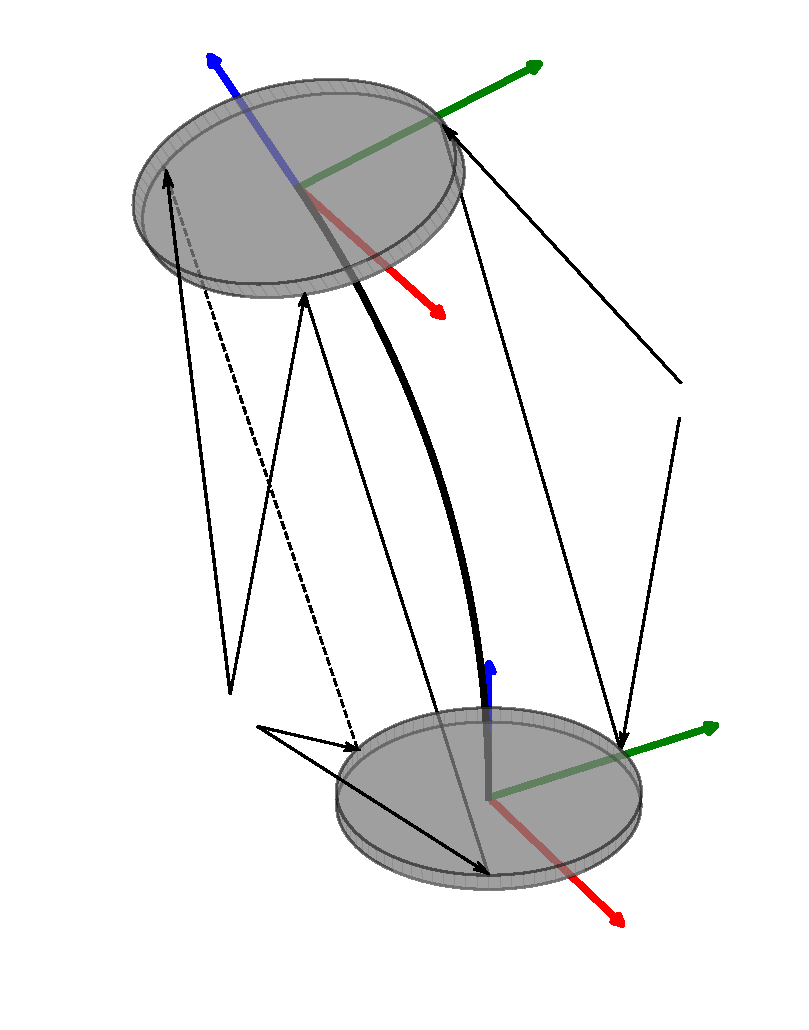
\includegraphics[width=.48\linewidth]{bilder/standdertechnik/continuum_robot3d.pdf}}
\begin{figure}[htb!]
\begin{subfigure}[t]{0.48\textwidth}
% füge bild ein, indem im Verhältnis zur definierten Box das Bild verschoben wird
\centering\raisebox{\dimexpr.5\ht\imagebox-.5\height}{
	\def\svgwidth{\textwidth}
	\input{bilder/standdertechnik/base.pdf_tex}
}
\caption{Trennscheibe der Roboterbasis}
\end{subfigure}
\begin{subfigure}[t]{0.48\textwidth}
\centering
\def\svgwidth{\textwidth}
\input{bilder/standdertechnik/continuum_robot3d.pdf_tex}
\caption{Segment des seilzugaktuierten kontinuierlichen Manipulators mit zwei Trennscheiben}
\end{subfigure}
\caption[Formgebung des Kontinuumsroboter durch Seilzüge]{Formgebung des Kontinuumsroboter durch Seilzüge}
\label{fig:roboterdesign}
\end{figure}

Die Krümmung des Kontinuumsroboters, bedingt durch die Seillängen und den Abstand der Seilführungen zum zentralen Rückgrat $d$, lautet
\begin{align}
\kappa = 2\frac{\sqrt{l_1^2+l_2^2+l_3^2-l_1l_2-l_2l_3-l_1l_3}}{d(l_1+l_2+l_3)}.
\label{eq:kappa}
\end{align}

Der Rotationswinkel des Kontinuumsroboters aus der $x$-$z$-Ebene wird durch
\begin{align}
\phi = \tan^{-1}\left(\frac{\sqrt{3}}{3} \frac{l_3+l_2-2l_1}{l_2-l_3} \right)
\label{eq:phi}
\end{align}

ermittelt. Für die numerische Berechnung des Rotationswinkels wird die Erweiterung der inversen Tangensfunktion $atan2(x, y)$, die die Vorzeichen der beiden Funktionsargumente $x$ und $y$ berücksichtigt, verwendet. Dadurch lässt sich der Rotationswinkel auf den Wertebereich von $[0~2\pi]$ abbilden. Zuletzt wird die Segmentlänge 
\begin{align}
\ell = \dfrac{nd(l_1+l_2+l_3)}{\sqrt{l_1^2+l_2^2+l_3^2-l_1l_2-l_2l_3-l_1l_3}} 
\sin^{-1}\left( \frac{\sqrt{l_1^2+l_2^2+l_3^2-l_1l_2-l_2l_3-l_1l_3}}{3nd} \right)
\label{eq:ell}
\end{align}

bestimmt. Die Anzahl der Trennscheiben beträgt $n$. Mit~\eqref{eq:kappa},~\eqref{eq:phi},~\eqref{eq:ell} wird an dieser Stelle die vektorwertige Funktion
\begin{align}
\bm{f}_{\mathrm{s}} =
\begin{bmatrix}
\kappa \\ \phi \\ \ell
\end{bmatrix} = 
\begin{bmatrix}
2\frac{\sqrt{l_1^2+l_2^2+l_3^2-l_1l_2-l_2l_3-l_1l_3}}{d(l_1+l_2+l_3)} \\
\tan^{-1}\left(\frac{\sqrt{3}}{3} \frac{l_3+l_2-2l_1}{l_2-l_3} \right) \\
\dfrac{nd(l_1+l_2+l_3)}{\sqrt{l_1^2+l_2^2+l_3^2-l_1l_2-l_2l_3-l_1l_3}} 
\sin^{-1}\left( \frac{\sqrt{l_1^2+l_2^2+l_3^2-l_1l_2-l_2l_3-l_1l_3}}{3nd} \right)
\end{bmatrix}
\label{eq:fspezifisch_vektor}
\end{align}

der Vollständigkeit halber angegeben. Zwischen zwei Trennscheiben wird angenommen, dass die Seilzüge keine Krümmung aufweisen. Erhöht man die Anzahl der Führungsscheiben theoretisch mit~$\lim n\to \infty$ entspricht dies einer Formgebung des Manipulators mit sich kontinuierlich krümmenden Aktoren~\cite{JW06}. Der Fall $l_1=l_2=l_3$ entspricht der singulären Stellung mit $\kappa = 0$, welcher für die Transformationsmatrix im vorigen Abschnitt bereits behandelt wurde. Für den Nennerterm des ersten Faktors von~\eqref{eq:ell} folgt dementsprechend: $\sqrt{l_1^2+l_2^2+l_3^2-l_1l_2-l_2l_3-l_1l_3} = 0$. Damit wäre die Berechnung der Segmentlänge im singulären Fall anhand~\eqref{eq:ell} nicht möglich. Die Segmentlänge entspricht hier der Länge der einzelnen Seilzüge \mbox{$\ell= (l_1+l_2+l_3)/3 = l_1=l_2=l_3$}.

Für die roboterspezifische Kinematik ist eine konstante Segmentlänge eine häufig gestellte Annahme. Dadurch lassen sich nur zwei Seillängen pro Segment unabhängig voneinander einstellen. Die dritte ist durch die Zwangsbedingung der konstanten Segmentlänge vorbestimmt. 
Im Rahmen dieser Arbeit weist die Kinematik eine variable Segmentlänge auf. Dadurch ist jedes einzelne Segment ein- und ausfahrbar. Die roboterspezifische Kinematik richtet sich damit maßgeblich nach~\cite{JW06a}. Die Autoren modellieren die Kinematik eines aus mehreren Segmenten bestehenden, seilzugaktuierten Kontinuumsroboters. Insbesondere werden Aktorgrenzen für die Gelenkwinkel berücksichtigt, die nicht durch eine konstante Segmentlänge eingeschränkt sind. Die einstellbaren \mbox{Gelenkwinkel $l_1, l_2, l_3$} werden durch eine untere und obere Grenze $l_{\mathrm{min}}$ bzw. $l_{\mathrm{max}}$ beschränkt. 

Seilzüge können prinzipiell nur Zugkräfte aufbauen und wären somit nicht in der Lage, den kontinuierlichen Manipulator über Aufbringen von Druckkräften zu strecken. Zwei Möglichkeiten, Druckkräfte zu entwickeln, werden an dieser Stelle erwähnt, aber im Weiteren für die Modellierung der Kinematik nicht weiter berücksichtigt. Eine Realisierung von Druckkräften ist prinzipiell mit einer am Rückgrat angebrachten Federvorrichtung möglich. Diese wird in Abhängigkeit von den eingestellten Gelenkwinkeln gestaucht oder gestreckt. Alternativ können die Seilzüge antagonistisch angeordnet werden, um Druckkräfte aufzubauen.  \newline

Mit den Ergebnissen der letzten beiden Abschnitte kann die gesamte, direkte kinematische Kette  
\begin{align}
\bm{x}_\mathrm{E} = \bm{f}_\mathrm{u} \left( \bm{f}_\mathrm{s} \left( [l_1, l_2, l_3]^\transpose \right) \right)
\label{eq:kinematische_kette}
\end{align}

eines seilzugaktuierten Kontinuumsroboters für ein Segment gebildet werden. Die Kinematik für mehrere verknüpfte Segmente eines Kontinuumsroboters ist Gegenstand des nächsten Abschnitts.

\subsection{Vorwärtskinematik mehrerer Segmente eines Kontinuumsroboters}
\label{subsec:multikinematik}

In den letzten beiden Abschnitten wurde der Grundstein für die direkte Kinematik eines seilzugaktuierten Kontinuumsroboter gelegt. Die Ergebnisse werden genutzt, um die Vorwärtskinematik des kontinuierlichen Manipulators mit mehreren verbundenen Segmenten zu ermitteln. \newline

Mit einer Verkettung von insgesamt $j$ homogenen Transformationsmatrizen
\begin{align}
{}^{0}\bm{T}_j = {}^{0}\bm{T}_{1} {}^1\bm{T}_{2} \dots {}^{j-1}\bm{T}_{j}
\end{align}

lässt sich eine beliebige Lage entlang von $j$ Segmenten transformieren. In dieser Arbeit werden zwei verknüpfte Segmente modelliert, sodass für die Transformationsmatrix folgt: ${}^{0}\bm{T}_2 = {}^{0}\bm{T}_{1} {}^1\bm{T}_{2}$. Sechs Gelenkwinkel 
$\bm{q} = \left[l_{1,1}, l_{1,2}, l_{1,3}, l_{2,1}, l_{2,2}, l_{2,3} \right]^\transpose$
beschreiben die Lage des Endeffektors eindeutig. 
Der erste Index der Seillängen bestimmt das Segment, an dem der Seilzug endet. Der Segmentindex steigt auf, beginnend bei der Roboterbasis. Der zweite Index legt den Seilzug gemäß Bild~\mbox{\ref{fig:roboterdesign}\,(b)} fest. Aus den gegebenen Seillängen des ersten Segments lässt sich die roboterspezifische Kinematik direkt berechnen. Die effektiven Seillängen des zweiten Segments, die für die Berechnung der Bogenparameter nötig sind, lauten
\begin{align}
l_{2,i,\mathrm{e}} = l_{2,i} - l_{1,i}\text{\,},~ i = 1,2,3.
\label{eq:effektive_laenge}
\end{align}

Die Seilzüge beider Segmente verlaufen jeweils durch dieselben Seilführungen der Trennscheiben. Es wird angenommen, dass die Seilzüge der jeweiligen Segmente die Formgebung des anderen Segments nicht beeinflussen. Dies stellt eine starke Vereinfachung dar, welche im Allgemeinen nicht gültig ist~\cite{WIJ10}. Diese Vereinfachung wird jedoch in Kauf genommen, da das Erlernen der inversen Kinematik mit Mitteln des RL im Vordergrund steht und nicht eine möglichst realistische Gestaltung der Kinematik beabsichtigt wird. \newline

Damit ist die Vorwärtskinematik für einen seilzugaktuierten Kontinuumsroboter mit zwei Segmenten vollständig beschrieben. Die Inverskinematik wird im nächsten Unterabschnitt behandelt.





\subsection{Inverskinematik}
\label{subesc:inverse_kinematik}

Für serielle Roboter wie auch Kontinuumsroboter gestaltet sich die Ermittlung der inversen Kinematik im Allgemeinen komplizierter als die der direkten. Zwei bestehende Konzepte zur Berechnung der inversen Kinematik eines kontinuierlichen Manipulators werden in diesem Abschnitt vorgestellt. Als erstes wird eine geometrische Ermittlung erläutert. Im Anschluss wird die differentielle Inverskinematik über die Berechnung von Jacobi-Matrizen vorgestellt. \newline

Ordnet man einer gegebenen Endeffektorlage eine Gelenkwinkelkonfiguration zu, spricht man von der Invers- bzw. inversen Kinematik
\begin{align}
\bm{q}  = \bm{f}^{-1} \left( \bm{x}_{\mathrm{E}} \right), 
\label{eq:inverskinematik}
\end{align} 

wobei $\bm{f}^{-1}$ die inverse Funktion zu $\bm{f}$ darstellt. In Hinblick auf Kontinuumsroboter mit stückweise konstanter Krümmung lässt sich die Inverskinematik in einen roboterunabhängigen Teil
\begin{align}
\left[ \kappa, \phi, \ell \right]^\transpose = \bm{f}^{-1}_{\mathrm{u}} \left( \bm{x}_{\mathrm{E}} \right)
\end{align}

und einen roboterspezifischen Teil
\begin{align}
\bm{q} = \bm{f}^{-1}_{\mathrm{s}} \left( \kappa, \phi, \ell \right)
\end{align}

aufteilen. Damit sind alle kinematischen Komponenten von Bild~\ref{fig:kinematikraeume} definiert. \newline

Zunächst wird die geometrische Lösung der inversen Kinematik erläutert.
Die inverse, roboterspezifische Funktion eines seilzugaktuierten Manipulators ist in~\cite{JW06} gegeben. Die Seillängen für ein Segment lassen sich geometrisch in Abhängigkeit der Kreisbogenparameter wie folgt berechnen:
\begin{align}
\bm{f}^{-1}_{\mathrm{s}} \left( \kappa, \phi, \ell \right) = 
\begin{bmatrix}
l_1 \\ l_2 \\l_3 
\end{bmatrix} =
\begin{bmatrix}
2n \sin \left( \dfrac{\kappa c}{2n} \right) \left( \dfrac{1}{\kappa} - d \sin\phi \right) \\
2n \sin \left( \dfrac{\kappa c}{2n} \right) \left( \dfrac{1}{\kappa} + d \sin \left(\dfrac{\pi}{3} + \phi  \right) \right) \\
2n \sin \left( \dfrac{\kappa c}{2n} \right) \left( \dfrac{1}{\kappa} - d \cos \left(\dfrac{\pi}{6} + \phi  \right) \right) \\
\end{bmatrix}.
\label{eq:fInversSpezifisch}
\end{align}

Damit ist prinzipiell nur noch die Bestimmung der inversen, roboterunabhängigen Kinematik notwendig. Es sind resultierende Kreisbogenparameter aus einer gegebenen Endeffektorlage gesucht. Neppalli et al. beschreiben in~\cite{NCJW09} ein Verfahren zur geometrischen Ermittlung von Kreisbogenparametern $\kappa, \phi, \ell$ aus einer gegebenen Endeffektorposition für einen Kontinuumsroboter mit $j$ Segmenten. Die Autoren lösen das beschriebene Problem mittels mehrerer Algorithmen, die in Tabelle~\ref{tab:geometrischeInverseUnabhaengigeKinematik} mit ihren Ein- und Ausgangsgrößen zusammengefasst sind. Die gewonnenen Bogenparameter können mit~\eqref{eq:fInversSpezifisch} in Seillängen des Kontinuumsroboters umgerechnet werden. 

Ein Nachteil der vorgestellten geometrischen Bestimmung von Bogenparametern besteht darin, dass die Abstände zwischen den Endpositionen der Robotersegmente vorgegeben werden müssen, siehe Tabelle~\ref{tab:geometrischeInverseUnabhaengigeKinematik}\,(a). Des Weiteren berücksichtigt dieser Ansatz keine Aktorgrenzen. Zuletzt ist die Orientierung des Endeffektors nicht Teil der Kinematik. 
\begin{table}[htb!]
\caption[Generelles Vorgehen der geometrischen Bestimmung von Kreisbogenparametern]
{Generelles Vorgehen der geometrischen Bestimmung von Kreisbogenparametern anhand einer gegeben Endeffektorlage nach~\cite{NCJW09}}
\begin{tabular}{ l  p{7.5cm} | p{6.50cm}}
\label{tab:geometrischeInverseUnabhaengigeKinematik}	
& \multicolumn{1}{c}{Eingangsgrößen} & \multicolumn{1}{c}{Ausgangsgrößen}\\ \hline\hline
(a) & Endeffektorposition $\bm{x}_{\mathrm{E,p}} = \bm{x}_{j,\mathrm{p}}$, Abstände zwischen den Endpositionen der einzelnen Robotersegmente \mbox{$d_i = ||\bm{x}_{i,\mathrm{p}}-\bm{x}_{i\shortminus1,\mathrm{p}}||_2$,} \mbox{$i = 1, \dots j $}, mit $\bm{x}_{0,\mathrm{p}} = \bm{0}$ & Endpositionen $\bm{x}_{i,\mathrm{p}}$, $i = 1,\dots j \shortminus 1$ \\ \hline
(b) & Endpositionen $\bm{x}_{i,\mathrm{p}}$, $i = 1, \dots j$, welche in die Roboterbasis transformiert werden &  Bogenparameter $\kappa_i, \phi_i, \ell_i$, $i \shortequal 1,  \dots j$ unter Anwendung von (c)  \\ \hline
(c) & Beliebige Position $\bm{x}_{\mathrm{p}}$ &  Bogenparameter $\kappa, \phi, \ell$ in Bezug zur Roboterbasis \\ 
\end{tabular}
\end{table}

Der nächste Ansatz löst die differentielle Kinematik
\begin{align}
\dot{\bm{x}}_{\mathrm{E}} = \bm{J} \mkern-1mu( \bm{q} ) \bm{q}
\label{eq:differentielle_kinematik}
\end{align}

mit der Jacobi-Matrix $\bm{J}\mkern-1mu (\bm{q})$. Über eine Invertierung der Jacobi-Matrix lässt sich die inverse, differentielle Kinematik 
\begin{align}
\dot{\bm{q}} = \bm{J}^{-1} \mkern-1mu( \bm{q} ) \dot{\bm{q}}
\label{eq:differentielleinverse_kinematik}
\end{align}

ermitteln. Nach~\cite{JW06} wird die folgende kinematischen Kette
\begin{align}
\bm{x}_{\mathrm{E}} 
\stackrel{\bm{f}_{\mathrm{DH}}}{\parbox{1cm}{\leftarrowfill}} \bm{\theta}, \bm{d}
\stackrel{\bm{f}_1}{\parbox{1cm}{\leftarrowfill}} \kappa, \phi, c
\stackrel{\bm{f}_2}{\parbox{1cm}{\leftarrowfill}} \bm{l}
\label{eq:informationsfluss_jones_walker}
\end{align}

aufgestellt. Die vektorwertige Funktion $\bm{f}_2$ entspricht dabei der bereits aufgeführten roboterspezifischen Kinematik gemäß~\eqref{eq:fspezifisch_vektor}, welche die Seillängen~$\bm{l}$ in Bogenparameter übersetzt. Die ermittelten Bogenparameter werden zunächst in klassische \textit{Denavit-Hartenberg}-Parameter~$\bm{\theta, \bm{d}}$ mittels $\bm{f}_1$ transformiert. Diese können wiederum mit~$\bm{f}_{\mathrm{DH}}$ zur \textit{Bishop}-Transformationsmatrix, gegeben durch~\eqref{eq:T_bishop}, überführt werden. Dieses Vorgehen unterscheidet sich von der Bestimmung der direkten, roboterunabhängigen Kinematik in Abschnitt~\ref{subsec:unabhaengige_vorwaertskinematik}, bei der die Transformationsmatrix direkt aus Bogenparametern ermittelt wird. Aus den einzelnen kinematischen Komponenten ermitteln die Autoren über eine Verkettung der Jacobi-Matrizen
\begin{align}
\dot{\bm{x}}_{\bm{\mathrm{E}}} = \bm{J}_{\mathrm{DH}} \bm{J}_{\bm{f}_1} \bm{J}_{\bm{f}_2}  \dot{\bm{l}} 
= \bm{J}\mkern-1mu (\bm{l}) \dot{\bm{l}}
\label{eq:modulare_differentielle_kinematik}
\end{align}

die differentielle Kinematik. Der modulare Aufbau der differentiellen Kinematik erlaubt es, diverse Hardware-Designs, die lediglich eine Anpassung der spezifischen Funktion $\bm{f}_2$ benötigen, zu realisieren. Außerdem ist eine echtzeitfähige Steuerung der Kinematik mit
\begin{align}
\dot{\bm{l}} = \bm{J}^{+} \mkern-2mu(\bm{l}) \dot{\bm{x}}
\label{eq:inverse_differentielle_kinematik}
\end{align}

möglich. $\bm{J}^{+}$, die Pseudoinverse zu $\bm{J}$, ist eine Verallgemeinerung der inversen Matrix auf singuläre und nichtquadratische Matrizen. \newline

Es wurden zwei Wege aufgezeigt, mit denen die inverse Kinematik eines seilzugaktuierten, kontinuierlichen Manipulators umgesetzt werden kann. Als nächstes wird das \textit{Reinforcement Learning} (RL) vorgestellt, bevor die in diesem Werk erarbeitete Methode der Inverskinematik von existierenden Ansätzen abgegrenzt wird.






\section{Reinforcement Learning}
\label{sec:rl_allgemein}

Wesentliche Konzepte, Komponenten und Begriffe des RL werden in diesem Abschnitt erläutert. RL umfasst eine Sammlung von Methoden des maschinellen Lernens und der künstlichen Intelligenz. Die Grundidee des RL besteht darin, Software- oder Roboteragenten zu gestalten, die durch Interaktionen mit einer unbekannten Umgebung über Versuch und Irrtum eigenständiges Handeln erlernen und definierte Ziele erreichen. \textit{Markow-Entscheidungsprozesse} (MEP) bilden die Grundlage für die Interaktion des Agenten mit einer unbekannten Umgebung und für die mathematische Analyse von RL-Algorithmen. Die Wertfunktion ermöglicht eine Bewertung von Zuständen, anhand welcher optimales Handeln abgeleitet werden kann. Die Strategie des Agenten, welche direkt ermittelt werden kann, ordnet Zuständen Aktionen zu. Der Agent versucht, seine Belohnungen in Form eines zukünftigen, diskontierten Ertrags zu maximieren. Die Standardmethoden des RL stoßen bei hochdimensionalen, kontinuierlichen Problemen an ihre Grenzen. Künstliche Neuronale Netze (KNN) verschaffen Abhilfe durch ihre Fähigkeit, hochdimensionale Zusammenhänge mit verhältnismäßig wenigen Parametern approximieren zu können. Werden neuronale Netze im Kontext des RL verwendet, spricht man von \textit{deep Reinforcement Learning} (dRL). Der grundlegende Aufbau sowie die Funktionsweise von neuronalen Netzen wird beschrieben. Drei Beispiele von erfolgreichen RL-Anwendungen sind in Bild~\ref{fig:rl_beispiele} illustriert. Bei der ersten Nennung von übersetzten Fachbegriffen ist nachstehend das englische Original angegeben. 

% ordne dem größten Bild eine Box zu
\newsavebox{\imgbox}
\savebox{\imgbox}{\includegraphics[width=0.32\textwidth]{bilder/standdertechnik/space_invaders.png}}
\begin{figure}[htb!]
\centering
\begin{subfigure}[t]{0.32\textwidth}
	\centering
	\includegraphics[width=\textwidth]{bilder/standdertechnik/space_invaders.png}
	\caption{\textit{Space Invaders}~\cite{MKS+15}}
\end{subfigure}
\begin{subfigure}[t]{0.32\textwidth}
	% erhöhe die Position der kleineren Bilder in Abhängigkeit von der Box
	\centering\raisebox{\dimexpr.5\ht\imgbox-.5\height}{
	\includegraphics[width=\textwidth]{bilder/standdertechnik/alphazero_go.png}
	}
	\caption{\textit{AlphaGo Zero}~\cite{SSS+17}}
\end{subfigure}
\begin{subfigure}[t]{0.32\textwidth}
	% erhöhe die Position der kleineren Bilder in Abhängigkeit von der Box
	\centering\raisebox{\dimexpr.5\ht\imgbox-.5\height}{
	\includegraphics[width=\textwidth]{bilder/standdertechnik/ball_in_cup.png}
	}
	\caption{Ball in Becher~\cite{NU11}}
\end{subfigure}
\caption[Anwendungen des Reinforcement Learning]{RL-Anwendungen. (a) Mithilfe des \textit{Deep Q-network} ist es möglich, Computerspiele direkt über die Auswertung von Pixeln zu lernen. Zu sehen ist das Spiel \textit{Space Invaders}. (b) \textit{AlphaGo Zero} ist eine künstliche Intelligenz, die ohne menschliches Expertenwissen das chinesische Brettspiel \textit{Go} gemeistert hat, indem sie unzählige Male gegen eine Kopie von sich selbst spielt. \textit{AlphaGo Zeros} Elo-Zahl liegt weit über den von den besten menschlichen Spielern.\footnotemark (c) Ein serieller Roboter lernt ein Geschicklichkeitsspiel, bei dem ein über eine Schnur verbundener Ball durch geschicktes Werfen in den Becher fallen soll.}
\label{fig:rl_beispiele}
\end{figure}




\pagebreak
\subsection{Markow-Entscheidungsprozesse und die Agent-Umgebung-Interaktion}
\label{subsec:MEP}



Wie eingangs erwähnt können RL-Probleme als MEP beschrieben werden. Alle Komponenten des MEP werden in dem Tupel 
$(\mathcal{S}, \mathcal{A}, \mathcal{T}, \mathcal{R}, \gamma)$
zusammengefasst. Nach~\cite{ADBB17} lauten die einzelnen Elemente:
%%%%%%%%%%%%%%%%%%%%%%%%%%%%%%%%%%%%%%%%%%%%%%%%%%%%%%%%%%%%%%%%%
\footnotetext{https://www.goratings.org/en/ (aufgerufen am 20.08.2018)}
%%%%%%%%%%%%%%%%%%%%%%%%%%%%%%%%%%%%%%%%%%%%%%%%%%%%%%%%%%%%%%%%%
\begin{itemize}
\item eine endliche Menge von Zuständen $\mathcal{S}$ (\textit{states}), sowie eine Verteilung von Ausgangszuständen~$\rho(\bm{s}_0)$
\item eine endliche Menge von Aktionen $\mathcal{A}$ (\textit{actions})
\item die Transitionsdynamik $\mathcal{T}( \bm{s}_{t+1} | \bm{s}_t, \bm{a}_t)$, die dem Zustand-Aktion-Paar (\textit{state action pair}) zur Zeit $t$ einen resultierenden Zustand zum Zeitpunkt $t+1$ zuordnet. Die Transitionsdynamik ist dem Agenten im Allgemeinen nicht bekannt
\item eine sofortige, skalare Belohnung, gegeben durch die Funktion $\mathcal{R}(\bm{s}_t, \bm{a}_t, \bm{s}_{t+1})$. Die Belohnung ist hervorgerufen durch die Aktion $\bm{a}_t$ im Zustand $\bm{s}_t$ und der folgenden Transition zum Zustand $\bm{s}_{t+1}$
\item der Diskontierungsfaktor (\textit{discount factor}) $\gamma \in [0~1]$, der zukünftige Belohnungen gewichtet
\end{itemize}



MEP werden in episodische und fortlaufende Prozesse unterteilt. Episodische MEP enden in einem finalen Zustand mit der Episodendauer $T$, wohingegen fortlaufende Prozesse die Episodendauer $T = \infty$ besitzen. In dieser Arbeit werden episodische MEP betrachtet. Zu jedem, diskreten Zeitpunkt $t = 0,1,2,3\dots,T$ beobachtet der Agent einen durch die Umgebung gegebenen Zustand $\bm{s}_t \in \mathcal{S}$. Ausgehend von diesem Zustand führt der Agent autonom und bedingt durch seine Strategie $\pi$ die Aktion $\bm{a}_t \in \mathcal{A}$ aus, welche die Umgebung beeinflusst. Die Strategie gibt formal die Wahrscheinlichkeitsverteilung für Aktionen in Abhängigkeit vom Zustand an: 
$\pi \, :\, \mathcal{S} \rightarrow p(\mathcal{A}=\bm{a}|\mathcal{S})$. 
Die Umgebung geht aufgrund der vom Agenten getätigten Aktion in den Zustand $\bm{s}_{t+1}$ über. Der neue Zustand sowie die instantane Belohnung $r_{t+1} \in \mathcal{R}$ werden an den Agenten kommuniziert. Im Rahmen von RL wird mit dem Belohnungssignal das Ziel oder ein für den Agenten beabsichtigtes Handeln definiert. Im Gegensatz zu Zuständen und Aktionen, die verallgemeinert als Vektorgrößen dargestellt sind, ist die Belohnung immer skalar.
In Bild~\ref{fig:agent_umgebung} ist der typische Signalflussplan der Agent-Umgebung-Interaktion veranschaulicht. RL ist verwandt mit dem Forschungsfeld der optimalen Regelung. Die Begriffe Agent, Umgebung, Aktion werden im RL anstatt der analogen Ausdrücke Regler, Regelstrecke und Stellgröße verwendet~\cite{SB98}.
\begin{figure}[!b]
\centering
\def\svgwidth{0.8\textwidth}
\input{bilder/standdertechnik/agent_umgebung.pdf_tex}
\caption[Agent-Umgebung-Interaktion]{Agent-Umgebung-Interaktion am Beispiel des Navigierens durch ein Labyrinth. Das Ziel ist, das Labyrinth durch den gegenüberliegenden Ausgang zu verlassen. Der Zustand $\bm{s}_t$ könnte die aktuelle Position des Agenten beschreiben. Planare Bewegungen \textit{oben}, \textit{unten}, \textit{links} und \textit{rechts} bilden ein simples Beispiel für mögliche Aktionen $\bm{a}_t$ im Labyrinth. Die Strategie $\pi$ bestimmt die Aktion des Agenten. Im Fall der vorliegenden Navigationsaufgabe ist das konstante Belohnungssignal $r_t= \shortminus 1$ ein beliebter Anreiz, den Agenten zum Verlassen des Labyrinths zu bewegen. Denn je länger der Agent sich im Labyrinth befindet, desto mehr negative Belohnungen erhält er. Diese können als Bestrafungen aufgefasst werden.}
\label{fig:agent_umgebung}
\end{figure}
Die Abfolge eines MEP lautet
\begin{align*}
\bm{s}_0, \bm{a}_0, r_1, \bm{s}_1, \bm{a}_1, r_1, \bm{s}_2, \bm{a}_2, r_3, \dots, T
\end{align*}

und wird Trajektorie genannt. Während jeder Trajektorie akkumuliert der Agent den diskontierten Ertrag (\textit{return})
\begin{align}
G = \sum_{t=0}^{T-1} \gamma^t r_{t+1},
\label{eq:ertrag}
\end{align}

den er zu maximieren versucht. Im Hinblick auf die Strategie lautet das Ziel von RL, eine optimale Strategie $\pi_*$ zu finden, die den maximalen erwarteten Ertrag erzielt $\pi_* = \argmax_\pi \mathds{E}[G|\pi]$.
In~\eqref{eq:ertrag} sind zwei Grenzfälle in Abhängigkeit des Diskontierungsfaktor zu erkennen. Für $\gamma=0$ fließt nur die instantane Belohnung in den Ertrag ein. Im Gegensatz dazu werden für $\gamma = 1$ alle Belohnungen unabhängig vom Zeitpunkt ihres Eintreffens gleich bewertet. Der Diskontierungsfaktor verringert im Allgemeinen zukünftige Belohnungen. In fortlaufenden MEP ist $\gamma < 1$ notwendig, damit die Summe~\eqref{eq:ertrag} einen endlichen Wert aufweist. 
MEP liegt die \textit{Markow-Eigenschaft} zugrunde, die besagt, dass zum Erreichen eines Ziels nur das Wissen über den aktuellen Zustand notwendig ist~\cite{SB98}. Zustände, die in der Vergangenheit liegen, beeinflussen damit die Entscheidungsfindung des Agenten nicht. Die Navigationsaufgabe des Agenten in Bild~\ref{fig:agent_umgebung} dient als Beispiel für die \textit{Markow-Eigenschaft} von RL-Problemen. Um an das Ende eines Labyrinths zu gelangen, spielt es für den Agenten keine Rolle, wo er sich in der Vergangenheit aufgehalten hat. \newline

In diesem Abschnitt wurden die elementaren Rahmenbedingungen vom RL erläutert. In dieser Arbeit werden zwei Klassen von Methoden zur Lösung von RL-Problemen behandelt. Die erste befasst sich mit der Ermittlung von Wertfunktionen. Die zweite errechnet parametrierte Strategien. Beide Klassen werden nachstehend beschrieben.






\subsection{Wertfunktionen}
\label{subsec:wertfunktionen}

Ein wesentlicher Bestandteil von RL ist die Wertfunktion (\textit{value function}), die Zustände bzw. Zustand-Aktion-Paare (\textit{state action pairs}) durch die Zuordnung eines Skalars bewertet. Nahezu alle RL-Algorithmen beinhalten die Schätzung einer Wertfunktion~\cite{SB98}. Aus diesem Grund werden die wesentlichen Aspekte von Wertfunktionen zusammengefasst. \newline

Die Zustand-Wertfunktion (\textit{state-value function})
\begin{align}
V_\pi(\bm{s}) = \mathds{E}[G|\bm{s},\pi]
\label{eq:zustand_wertfunktion}
\end{align}

entspricht dem erwarteten Ertrag~\eqref{eq:ertrag}, wenn sich der Agent im Zustand $\bm{s}$ befindet und der Strategie $\pi$ folgt. Die Zustand-Wertfunktion ist ein allgemeines Maß dafür, welcher diskontierte, zukünftige Ertrag in bestimmten Zuständen zu erwarten ist. 
Die Zustand-Aktion-Wertfunktion, auch Q-Funktion genannt, (\textit{state-action-value function}) 
\begin{align}
Q_\pi (\bm{s}, \bm{a}) = \mathds{E}[G|\bm{s},\bm{a},\pi]
\label{eq:zustand_aktion_wertfunktion}
\end{align}

ähnelt~\eqref{eq:zustand_wertfunktion}. Der einzige Unterschied besteht darin, dass in~\eqref{eq:zustand_aktion_wertfunktion} eine auszuführende Aktion $\bm{a}$ im Zustand $\bm{s}$ gegeben ist. Nach Ausführung der Aktion wird die Strategie $\pi$ verfolgt.
Die optimale Strategie $\pi_*$ maximiert den erwarteten, zukünftigen Ertrag
\begin{align}
V_*	(\bm{s}) = \max\limits_{\pi} V_\pi (\bm{s}) \quad \forall \, \bm{s} \in \mathcal{S}.
\label{eq:v_optimal}
\end{align}

Ist $V_*(\bm{s})$ bekannt, wählt der Agent im Zustand $\bm{s}$ die Aktion $\bm{a}$, die $\mathds{E}[V_*(\bm{s}_{t+1})]$ maximiert.  Die optimale Strategie bezüglich der Zustand-Aktion-Wertfunktion wählt die Aktion $\bm{a}$ gierig (\textit{greedy}) im Hinblick auf alle vorhandenen Aktionen im Zustand $\bm{s}$:
$\argmax_{\bm{a}} Q_\pi (\bm{s}, \bm{a})$. Die $\argmax$-Funktion ermittelt die Aktion $\bm{a}$, die den ihr folgenden, mathematischen Ausdruck maximiert. Eine weitere wichtige Größe in RL-Algorithmen ist der Vorteil (\textit{advantage})
\begin{align}
A_\pi (\bm{s},\bm{a}) = Q_\pi(\bm{s}, \bm{a}) - V_\pi (\bm{s}). 
\label{eq:vorteil}
\end{align}

Im Gegensatz zu~\eqref{eq:zustand_wertfunktion} und~\eqref{eq:zustand_aktion_wertfunktion} gibt der Vorteil nicht einen absoluten, sondern einen relativen Wert an. Der Vorteil gibt darüber Auskunft, inwiefern die vom Agenten gewählten Aktion $\bm{a}$ ihn im Zustand $\bm{s}$ besser oder schlechter stellt. 

Die Methoden des dynamischen Programmierens ermöglichen im tabellarischen Fall, RL-Probleme rekursiv zu lösen. Hierbei wird die Markow-Eigenschaft genutzt, um die Zustand-Wertfunktion in Form einer Bellman-Gleichung
\begin{align}
V_\pi (\bm{s}_t) = \max\limits_{\bm{a}} \mathds{E}[r_{t+1} + \gamma V_\pi(\bm{s}_{t+1})]
\label{eq:bellman_v}
\end{align}

zu definieren. Ausgehend vom Zustand~$\bm{s}_t$ wird diejenige Aktion gewählt, die den Erwartungswert der sofortigen Belohnung sowie den diskontierten Wert des folgenden Zustands~$\bm{s}_{t+1}$ maximiert. Die Bellman-Gleichung für die Zustand-Aktion-Wertfunktion lautet:
\begin{align}
Q_\pi (\bm{s}_t, \bm{a}_t) = \mathds{E} \left[r_{t+1} + \gamma \max\limits_{\bm{a}_{t+1}} Q_\pi (\bm{s}_{t+1}, \pi(\bm{s}_{t+1})) \right].
\label{eq:bellman_q}
\end{align}

Die Gleichungen~\eqref{eq:bellman_v} und~\eqref{eq:bellman_q} werden mit der Methode des \textit{Bootstrapping} ermittelt. Das heißt, es wird eine aktuelle Schätzung der Wertfunktionen verwendet, um eine Verbesserung der jeweiligen Schätzungen zu bewerkstelligen. 

Die generalisierte Strategieiteration (\textit{generalized policy iteration}) beschreibt das Vorgehen zum Auffinden der optimalen Wertfunktion. Eine Iteration der Strategie besteht aus der Strategieevaluation (\textit{strategy evaluation}) und der Strategieverbesserung (\textit{strategy improvement}). Strategieevaluation schätzt die Wertfunktion für eine beliebige Strategie $\pi$. Eine Strategieverbesserung kann durch gieriges Handeln hinsichtlich der Wertfunktion erzielt werden. Das heißt der Agent wählt Aktionen, die den maximalen, erwarteten Ertrag zur Folge haben. 

Im tabellarischen Fall müsste man prinzipiell für jeden Zustand einen Eintrag im Speicher hinterlegen. Für Probleme mit wenigen Zuständen sind tabellarische Methoden in der Lage, optimale Lösungen zu finden. Sobald man jedoch versucht kontinuierliche Probleme zu lösen, ist die computergestützte, tabellarische Repräsentation von Zuständen nicht mehr realisierbar. 
%Das Spiel \textit{GO} weist beispielsweise $~2 * 10^170$ erlaubte Positionen auf. 
Aus diesem Grund werden Methoden der Funktionsapproximation herangezogen, die in Abschnitt~\ref{sec:knn} erläutert werden.\newline

Mithilfe von Wertfunktionen lassen sich Zustände bewerten und schließlich optimales Handeln des Agenten ableiten. Die zweite Methode, RL-Probleme zu lösen, folgt im nächsten Unterabschnitt.






\subsection{Strategiesuche}
\label{subsec:strategiesuche}

Bei der Strategiesuche wird direkt eine optimale Strategie gesucht, anstatt diese über die Ermittlung der Wertfunktion abzuleiten. Strategien werden üblicherweise mit einem Satz von Parametern $\bm{\theta}$ beschrieben. Eine parametrierte Strategie $\pi_{\bm{\theta}}$ wählt Aktionen hinsichtlich ihrer Parameter und wird mit dem entsprechenden Subskript versehen. Das Ziel der Strategiesuche besteht darin, den erwarteten Ertrag 
$\mathds{E}[G|\bm{\theta}]$ 
durch entsprechende Parameteraktualisierungen zu maximieren. Es existieren gradientenfreie und gradientenbasierte Verfahren zur Optimierung von parametrierten Strategien, wobei letztere im Vordergrund dieser Arbeit stehen. \newline

Strategien $\pi(\bm{a}|\bm{s},\bm{\theta})$ können prinzipiell beliebig parametriert werden, solange sie differenzierbar hinsichtlich ihrer Parameter sind. Folglich existiert der Gradient $\nabla_{\bm{\theta}}\pi(\bm{a}|\bm{s},\bm{\theta})$ und ist endlich, mit $\nabla_{\bm{\theta}}$, dem Nabla-Operator hinsichtlich der Parameter $\bm{\theta}$.  Die gradientenbasierte Parameteraktualisierung wird mittels des Gradientenaufstiegs (\textit{gradient ascent})
\begin{align}
\bm{\theta}_{t+1} = \bm{\theta}_t + \alpha \nabla_{\bm{\theta}} \bm{L}(\bm{\theta}_t)
\label{eq:parameterupdate}
\end{align}

bewerkstelligt. Die Kostenfunktion $\bm{L}(\bm{\theta})$ beinhaltet meist eine Form des erwarteten Ertrags sowie der parametrierten Strategie. Die Lernrate $\alpha$ skaliert die Parameteraktualisierung und nimmt üblicherweise einen Wert $\alpha \ll 1$ an. Strategiegrandientenmethoden (\textit{policy gradient methods}) werden alle Verfahren genannt, welche die Parameteraktualisierung~\eqref{eq:parameterupdate} verwenden. 
Die Ausgangsgrößen von stochastischen Strategien (\textit{stochastic policies}) berechnen die Parameter einer Wahrscheinlichkeitsverteilung, z.\,B. den Erwartungswert und die Standardabweichung der Gaußschen Normalverteilung. Damit ist die Strategie in der Lage, Werte für die Aktionen des Agenten direkt zu errechnen. 

Das gradientenbasierte Strategie-Theorem (\textit{policy gradient theorem}) liefert einen analytischen Ausdruck für den Gradienten der Kostenfunktion hinsichtlich ihrer Parameter~\cite{SB98}. Die Parameteraktualisierung des REINFORCE-Algorithmus~\cite{Wil92} 
\begin{align}
\bm{\theta}_{t+1} = \bm{\theta}_t + \alpha G_t 
\dfrac{\nabla_{\bm{\theta}} \pi(\bm{a}_t|\bm{s}_t, \bm{\theta}_t)}{\pi(\bm{a}_t|\bm{s}_t, \bm{\theta}_t)}
\label{eq:REINFORCE}
\end{align}

wird aufgrund ihrer veranschaulichenden Wirkung beispielhaft aufgeführt. Die Parameterveränderung ist proportional zu dem Produkt aus dem Ertrag $G_t$ und einem Vektor, dem Gradienten der Wahrscheinlichkeit, eine Aktion auszuführen, dividiert durch die Wahrscheinlichkeit, die Aktion zu wählen. Der Vektor zeigt in die Richtung des steilsten Anstiegs im Parameterraum, dieselbe Aktion im selben Zustand zu wiederholen. Das heißt, \eqref{eq:REINFORCE} verändert die Wahrscheinlichkeit von Aktionen proportional zum Ertrag. Aktionen, die einen geringen Ertrag liefern, werden nach der Parameteraktualisierung unwahrscheinlicher gemacht. Wiederum wird die Wahrscheinlichkeit von Aktionen, die einen hohen Ertrag erzielen, erhöht. Der Ausdruck im Nenner sorgt dafür, dass seltene Aktionen berücksichtigt werden. Ansonsten werden wahrscheinlich eintretende Aktionen mit möglicherweise geringem Ertrag bevorzugt. \newline

Wertfunktionen sowie Strategien kontinuierlicher und hochdimensionaler RL-Probleme werden parametriert und approximiert. Künstliche neuronale Netze stellen eine Möglichkeit dar, Funktionen zu approximieren.





\section{Künstliche neuronale Netzwerke}
\label{sec:knn}

Der Gebrauch von KNN in Verbindung mit RL ermöglicht das Lösen von komplizierten, hochdimensionalen Problemen~\cite{ADBB17}. Die Fähigkeit von KNN, komplexe Zusammenhänge mit relativ wenigen Parametern repräsentieren zu können, spielt hierbei eine bedeutende Rolle.  
%Besondere Erfolge wurden in der Bildverarbeitung, Spracherkennung und -übersetzung verbucht~\cite{GBC16}. 
%Im Folgenden werden die grundlegenden Elemente und Funktionsweisen eines KNN dargelegt. 
In diesem Abschnitt wird zunächst der generelle Aufbau von KNN erläutert. Anschließend werden einige wichtige Aktivierungs- bzw. Transformationsfunktionen vorgestellt. Der \textit{Backpropagation}-Algorithmus, nachfolgend \textit{Backpropagation} genannt, wird verwendet, um das Erlernen von Zusammenhängen durch KNN zu ermöglichen. 






\subsection{Netzwerkarchitektur und Vorwärtspass}
\label{subsec:architektur_vorwaertspass}

In Verbindung mit RL stechen zwei häufig applizierte Netzwerkarchitekturen hervor: neuronale Vorwärtsnetzwerke (\textit{feedforward neural nets}) und neuronale Faltungsnetzwerke (\textit{convolutional neural nets}). Die Architektur bestimmt die Funktionsweise des Netzwerks. Vorwärtsnetzwerke errechnen die formale Beziehung
$\bm{y} = f(\bm{x};\bm{\theta})$,
welche den funktionalen Zusammenhang zwischen dem Eingangssignal $\bm{x}$ und dem Ausgangssignal $\bm{y}$ approximiert. Die zu lernenden Parameter sind $\bm{\theta}$. Werden Vorwärtsnetzwerke zusätzlich mit Faltungsschichten (\textit{convolutional layers}) versehen, spricht man von Faltungsnetzwerken. In der Bild- und Sprachverarbeitung ist die Verwendung von Faltungsoperationen relevant, da dadurch niedrigdimensionale Merkmale (\textit{features}) aus hochdimensionalen Daten extrahiert werden können. Nachfolgend wird der Fokus auf Vorwärtsnetzwerke gelegt. 
\newline

Vorwärtsnetzwerke besitzen eine Eingangs- und Ausgangsschicht (\textit{input and output layer}) sowie mindestens eine versteckte Schicht (\textit{hidden layer}). Bild~\ref{fig:knn} illustriert ein flaches Vorwärtsnetzwerk mit einer versteckten Schicht. Jeder Kreis repräsentiert ein Neuron, die kleinste Einheit des KNN. Ein Netz heißt dicht oder dicht vernetzt, wenn alle Neuronen einer Schicht Verbindungen zu allen Neuronen der folgenden Schicht aufweisen. Tiefe Vorwärtsnetzwerke besitzen mindestens zwei versteckte Schichten. 
\begin{figure}[h]
\centering
\def\svgwidth{0.7\textwidth}
\input{bilder/standdertechnik/knn.pdf_tex}
\caption[Dicht vernetztes, flaches Vorwärtsnetzwerk]{Dicht vernetztes, flaches Vorwärtsnetzwerk}
\label{fig:knn}
\end{figure}

Während die Dimensionalität des Ein- und Ausgangssignals durch äußere Rahmenbedingungen vorgegeben ist, hängt die Dimension der Wichtungsmatrizen $\bm{W}$ und Voraktivierungen $\bm{b}$ von der gewählten Anzahl der Neuronen ab. Neuronen sind skalare Matrix- bzw. Vektoreinträge, die während des Trainings des Netzes angepasst werden, sodass sie definierte Kostenfunktionen maximieren oder minimieren. Das Eingangssignal wird durch das Netzwerk mittels Matrix-Vektormultiplikation und Aktivierungsfunktionen geleitet und transformiert, sodass schließlich das Ausgangssignal errechnet wird. Dieser Vorgang nennt sich Vorwärtspass (\textit{forward pass}) und ist in Algorithmus~\ref{alg:vorwaertspass} mit seinen mathematischen Operationen aufgeführt. 
\begin{algorithm}[!htb]
\caption[Vorwärtspass eines dicht vernetzten Vorwärtsnetzwerks]{Vorwärtspass eines dicht vernetzten Vorwärtsnetzwerks in Anlehnung an~\cite{GBC16}. Die zu lernenden Parameter $\bm{\theta}$ sind in den Wichtungsmatrizen $\bm{W}_i$ und den Voraktivierungen $\bm{b}_i$ (\textit{bias}) enthalten. Nach einer Multiplikation des vektorwertigen Signals $\bm{h}_{i-1}$ mit der Wichtungsmatrix $\bm{W}_i$ wird die Voraktivierung $\bm{b}_i$ addiert. Die resultierende Summe wird durch die nichtlineare Aktivierungsfunktion $g(\bm{z}_i)$ transformiert. Dieser Vorgang wird solange wiederholt, bis alle Schichten des Netzwerks passiert sind und das Ausgangssignal $\bm{y}$ ermittelt ist.}
\label{alg:vorwaertspass}
\begin{algorithmic}[1]
\Require Netzwerktiefe $k$
\Require Wichtungsmatrizen $\bm{W}_i, i \in \{1, \dots, k\}$
\Require Voraktivierungen $\bm{b}_i, i \in \{1, \dots, k\}$
\Require Aktivierungsfunktionen $g_i(\bm{z}), i \in \{1, \dots, k\}$
\Require Eingangssignal $\bm{x}$
\State $\bm{h}_0 = \bm{x}$
\For{i=1, \dots, k} 
%	\State $\bm{z}_i = \bm{b}_i + \bm{W}_i \bm{h}_{i-1}$
	\State $\bm{h}_i = g_i(\bm{W}_i \bm{h}_{i-1} + \bm{b}_i)$
\EndFor
\State $\bm{y} = \bm{h}_k$
\end{algorithmic}
\end{algorithm}







\subsection{Nichtlineare Aktivierungen}
\label{subsec:nichtlineare_aktivierung}

Ein entscheidender Vorgang des Vorwärtspasses bildet die nichtlineare Aktivierung, welche die Approximation von nichtlinearen Zusammenhängen erst ermöglicht, da der Vorwärtspass sonst nur aus einer Kombination von linearen Funktion bestehen würde. In diesem Unterabschnitt werden drei relevante Aktivierungsfunktionen vorgestellt. \newline

\textit{Rectified linear units} (ReLU) besitzen die Aktivierungsfunktion $g(z) = max\{0,z\}$ und werden von Goodfellow et al. als Standardaktivierungen für die versteckten Schichten von KNN vorgeschlagen. ReLU bilden eine stückweise lineare Funktion, wodurch sie viele Eigenschaften bewahren, die die Optimierung mittels gradientenbasierter Verfahren vereinfacht~\cite{GBC16}.

Die nichtlineare Aktivierung der Ausgangsschicht ist optional und hängt von dem zu approximierenden Sachverhalt ab. Für Klassifizierungsprobleme mit nur zwei Kategorien kann die logistische Sigmoidfunktion $g(z) = 1/(1+\exp(-z))$ eingesetzt werden.
Sigmoidfunktionen bilden eine Klasse von Funktionen mit S-förmigen Graphen. Die logistische Sigmoidfunktion besitzt den Wertebereich $g(z)\in[ 0~1]$, wodurch das Ergebnis als Wahrscheinlichkeit, eine von zwei Klassen identifiziert zu haben, interpretiert werden kann. 


Möchte man mit einem KNN bspw. ein Beschleunigungs- oder Bremssignal mithilfe eines Skalars approximieren, wobei positive Werte eine Beschleunigung und negative eine Bremsung hervorrufen, kann man den Tangens hyperbolicus als Aktivierungsfunktion verwenden. Dieser liefert Werte zwischen $\shortminus 1$ und $1$. 

Die drei vorgestellten Aktivierungsfunktionen sind in Bild~\ref{fig:aktivierungen} dargestellt. 
Das universale Approximationstheorem (\textit{universal approximation theorem}) besagt, dass ein Vorwärtsnetzwerk mit einer versteckten Schicht, einer nichtlinearen Aktivierung und einer finiten Anzahl von Neuronen beliebige, kontinuierliche Funktionen approximieren kann. 
Für Sigmoidfunktionen hat Cybenko in~\cite{Cyb89} und für ReLU haben Leshno et al. in~\cite{LLPS93} das Theorem nachgewiesen.

\begin{figure}[!htb]
\centering
\begin{subfigure}{.32\textwidth}
	\centering
	\begin{tikzpicture}
	\begin{axis}[xmax=3, xmin=-3, ymax=1, ymin=-1, samples=50, width=\textwidth]
		\addplot[imesblue, ultra thick][domain=-3:0] {0};
		\addplot[imesblue, ultra thick][domain=0:3] {x};
	\end{axis}	
	\end{tikzpicture}
	\caption{ReLU}
\end{subfigure}
\begin{subfigure}{.32\textwidth}
	\centering
	\begin{tikzpicture}
	\begin{axis}[xmax=3, xmin=-3, ymax=1, ymin=-1, samples=50, width=\textwidth]
		\addplot[imesblue, ultra thick] {1/(1+ exp(-x) )};
	\end{axis}	
	\end{tikzpicture}
	\caption{Logistische Sigmoidfunktion}
\end{subfigure}
\begin{subfigure}{.32\textwidth}
	\centering
	\begin{tikzpicture}
	\begin{axis}[xmax=3, xmin=-3, ymax=1, ymin=-1, samples=50, width=\textwidth]
		\addplot[imesblue, ultra thick] {tanh(x)};
	\end{axis}	
	\end{tikzpicture}
	\caption{Tangens hyperbolicus}
\end{subfigure}
\caption{Drei relevante Aktivierungsfunktionen}
\label{fig:aktivierungen}
\end{figure}





\subsection{Backpropagation}
\label{subsec:backprop}

Wie bereits erwähnt werden Wertfunktionen oder Strategien im RL mit KNN approximiert. 
Ein KNN, welches eine Strategie repräsentiert, errechnet im Vorwärtspass aus einem Zustand des Agenten die dazugehörige Aktion. Die ermittelte Aktion hat Auswirkungen auf den resultierenden Ertrag und folglich auch auf die Parameteraktualisierung und Kostenfunktion in~\eqref{eq:parameterupdate} bei der Strategiesuche. Das Ziel der Strategiesuche besteht darin, die Parameter $\bm{\theta}$ zu erlernen, die den zukünftigen, erwarteten Ertrag maximieren. Dafür wird der Gradient der Kostenfunktion hinsichtlich der zu lernenden Parameter benötigt. 
Backpropagation wird verwendet, um Informationen rückwärts durch das Netzwerk fließen zu lassen und die notwendigen Gradienten zu ermitteln. 
Formal ermittelt Backpropagation den Gradienten $\nabla_{\bm{\theta}} \bm{L}(\bm{\theta})$ unter Anwendung der Kettenregel der Differentiation. Auf eine detaillierte Beschreibung von Backpropagation wird an dieser Stelle verzichtet, da Software-Bibliotheken des maschinellen Lernens eigenständig den Gradienten der Kostenfunktion in Abhängigkeit vom Vorwärtsnetzwerk ermitteln können. Für die Lösung eines RL-Problems steht die Gestaltung des Vorwärtspasses dabei im Vordergrund. \newline

		%\chapter{Modellierung der direkten Kinematik}

In diesem Kapitel wird die direkte Kinematik eines seilzugaktuierten Kontinuumroboters bestehend aus zwei Abschnitten aufgestellt. Im Allgemeinen bezeichnet die direkte Kinematik 
%
\begin{equation}
\label{eq:direkteKinematik}
f(\bm{q}) = \bm{x}_\mathrm{E}
\end{equation}
%
den geometrischen Zusammenhang zwischen den $m$ Gelenkwinkeln $\bm{q} = \left[q_1, q_2, ..., q_m \right]^\transpose $ des Roboters und der daraus resultierenden Position und Lage Endeffektors~$\bm{x}_\mathrm{E}$.
$\bm{x}_\mathrm{E} = \left[x_\mathrm{E}, y_\mathrm{E}, z_\mathrm{E}, \phi_\mathrm{E}, \psi_\mathrm{E}, \theta_\mathrm{E} \right]^\transpose $. Hierbei entspricht $m$ der Anzahl der Gelenkwinkel und $\bm{x}_\mathrm{E}$ den kartesischen Raumkoordinaten sowie der Orientierung des Endeffektors. Die Orientierung ist hier zunächst durch die Verwendung von drei Winkeln $\phi_\mathrm{E}, \psi_\mathrm{E}$ und $\theta_\mathrm{E}$ dargestellt. 
Die direkte Kinematik lässt sich auf die Gelenkwinkelgeschwindikeiten $f(\bm{\dot{q}}) = \bm{\dot{x}}_\mathrm{E} $ und -beschleunigungen $f(\bm{\ddot{q}}) = \bm{\ddot{x}}_\mathrm{E}$ erweitern. Im späteren Verlauf dieser Arbeit wird die inverse Kinematik
%
\begin{align}
f^{-1}(\bm{x}_\mathrm{E}) = \bm{q},
\label{eq:inverseKinematik}
\end{align}

\begin{figure}[b]
\centering
\begin{tikzpicture}[auto, node distance=2cm, line width=2pt]
% Zeichne Blöcke mit innerem Text
\node[name=center] {};
\node[simplebox, minimum size=1.5cm, left of=center, name=q, color=imesblue, label={[align=center]:Gelenk-\\ winkel}, label={[align=center]below:Gelenk-\\ raum}] {\textblack{$\bm{q}$}};
\node[simplebox, minimum size=1.5cm, right of=center, name=x, label={[align=center]:Position,\\ Lage}, label={[align=center]below:Arbeits-\\ raum}] {\textblack{$\bm{x}_\mathrm{E}$}};
% berechne Punkte für verschobene Linien zwischen Boxen
\path (q.east) -- (q.north east) coordinate[pos=0.5] (q1);
\path (q.east) -- (q.south east) coordinate[pos=0.5] (q2);
\path (x.west) -- (x.north west) coordinate[pos=0.5] (x1);
\path (x.west) -- (x.south west) coordinate[pos=0.5] (x2);
%Zeichne Verbindungen
\draw[simplearrow] (q1) to node [align=center] {\textblack{$f(\bm{q})$}}      (x1);
\draw[simplearrow] (x2) to node [align=center] {\textblack{$f^{-1}(\bm{x}_\mathrm{E})$}} (q2);

\end{tikzpicture}
\caption{Grafische Darstellung der direkten und inversen Kinematik}
\label{fig:kinematik}
\end{figure}

welche eine gegebene Lage und Orientierung im Arbeitsraum Gelenkwinkel zuordnet, ermittelt. Die Beziehung zwischen der direkten und inversen Kinematik ist in \abb{fig:kinematik} grafisch dargestellt. 

Im Gegensatz zu seriellen Robotern mit starren Strukturen besitzen Kontinuumsroboter ein nachgiebiges Glied, welches sich kontinuierlich unter dem Einfluss von Kräften krümmt. Für die Modellierung der direkten Kinematik wird im Rahmen dieser Arbeit die Annahme getroffen, dass der Kontinuumroboter in jedem Abschnitt eine stückweise konstante Krümmung annimmt. Damit lässt sich die Form jedes Abschnitts mithilfe eines Kreisbogens beschreiben. Dies ermöglicht weiterhin die Kinematik von Kontinuumrobotern in einen roboterspezifischen und einen roboterunabhängigen Zusammenhang aufzuteilen \cite{WIJ10}. Unter Verwendung der Gelenkwinkel ermittelt die roboterspezifische Funktion
%
\begin{align}
f_{\mathrm{s}}(\bm{q}) = [\kappa, \phi, l]^\transpose
\label{eq:fspezifisch}
\end{align}

die sogenannten Bogenparameter im Konfigurationsraum. Es sind $\kappa$ die Krümmung eines stückweise konstant gekrümmten Abschnitts des Kontinuumroboters, $\phi$ der Winkel der Ebene, in welcher der Kreisbogen liegt, und $l$ die Länge des Kreisbogens. Um sämtliche Punkte auf dem Kreisbogen beschreiben zu können, wird die variable Bogenlänge $s \in [0~l]$ eingeführt. Analog zu \eqref{eq:inverseKinematik} lässt sich auch die inverse Abbildung
%
\begin{align}
f^{-1}_{\mathrm{s}}(\kappa, \phi, l) = \bm{q}
\label{eq:fspezifischinvers}
\end{align}

vom Konfigurationsraum zum Gelenkraum definieren. Der roboterunabhängige Zusammenhang 
%
\begin{align}
f_{\text{u}}(\kappa, \phi, l) = \bm{x}_\mathrm{E}
\label{eq:funabhängig}
\end{align}

bildet über die Bogenparameter den Konfigurationsraum auf den Arbeitsraum ab. Der Zusammenhang zwischen den roboterspezifischen und -unabhängigen Abbildungen ist in~\abb{fig:kinematikraeume} zu sehen. In den folgenden Unterkapiteln wird zunächst die roboterunabhängige und dann die roboterspezifische Kinematik von einem konstant gekrümmten Abschnitt für einen seilzugaktuierten Kontinuumsroboter aufgestellt. Mit den gewonnenen Ergebnissen kann im Anschluss über die Kopplung zweier homogener Transformationen die Kinematik auf zwei Abschnitte erweitert werden. \\

 
\begin{figure}[b] % 
\centering
\begin{tikzpicture}[auto, node distance=4cm]
% Erzeuge Boxen mit innerem Text
\node[simplebox, minimum size=1.5cm, name=arcparams, label={[align=center]:Bogen-\\ parameter}, label={[align=center]below:Konfigurations-\\ raum}] {\textblack{$\kappa, \phi, l$}};
\node[simplebox, minimum size=1.5cm, node distance=5cm, left of=center, name=q, label={[align=center]:Seil-\\ längen}, label={[align=center]below:Gelenk-\\ raum}] {\textblack{$\bm{q}$}};
\node[simplebox, minimum size=1.5cm, node distance=5cm, right of=center, name=x, label={[align=center]:Position,\\ Orientierung}, label={[align=center]below:Arbeits-\\ raum}] {\textblack{$\bm{x}_\mathrm{E}$}};
% berechne Punkte für verschobene Linien zwischen Boxen
\path (arcparams.east) -- (arcparams.north east) coordinate[pos=0.5] (arcparamsright1);
\path (arcparams.east) -- (arcparams.south east) coordinate[pos=0.5] (arcparamsright2);
\path (arcparams.west) -- (arcparams.north west) coordinate[pos=0.5] (arcparamsleft1);
\path (arcparams.west) -- (arcparams.south west) coordinate[pos=0.5] (arcparamsleft2);
\path (q.east) -- (q.north east) coordinate[pos=0.5] (q1);
\path (q.east) -- (q.south east) coordinate[pos=0.5] (q2);
\path (x.west) -- (x.north west) coordinate[pos=0.5] (x1);
\path (x.west) -- (x.south west) coordinate[pos=0.5] (x2);
% zeichne Pfeile zwischen den Boxen
\draw[simplearrow] (q1) to node [align=center] {\textblack{$f_{\text{s}}(\bm{q})$}}      (arcparamsleft1);
\draw[simplearrow] (arcparamsleft2) to node [align=center] {\textblack{$f^{-1}_{\text{s}}(\kappa, \phi, l)$}} (q2);
\draw[simplearrow] (x2) to node [align=center] {\textblack{$f^{-1}_{\text{u}}(\bm{x}_\mathrm{E})$}}      (arcparamsright2);
\draw[simplearrow] (arcparamsright1) to node [align=center] {\textblack{$f_{\text{u}}(\kappa, \phi, l)$}} (x1);

\end{tikzpicture}
\caption[Grafische Darstellung der unterschiedlichen Arbeitsräume eines Kontinuumsroboters]{Grafische Darstellung der unterschiedlichen Arbeitsräume eines Kontinuumsroboters in Anlehnung an \cite{WIJ10}}
\label{fig:kinematikraeume}
\end{figure}

\section{Die roboterunabhängige Kinematik}
\label{sec:unabhängigeKinematik}

Erkläre hier, dass $f^{-1}_\mathrm{s}$ von Bogenparametern zu Seillängen bekannt ist~\cite{JW06}.


INSERT GRAPHIC HERE VON WEGEN MIT EINEM KREISBOGEN UND DEN PARAMETERN UND DEN KOORDINATEN
\section{Die roboterspezifische Kinematik}
\label{sec:spezifischeKinematik}

Die roboterspezifische Kinematik stellt den direkten Zusammenhang zwischen den entsprechenden Gelenkwinkeln im Gelenkraum und den Bogenparametern im Konfigurationsraum her. Die auf die Roboterstruktur wirkenden Kräfte und Momente der Aktuatoren sind für die tatsächliche Formgebung relevant. Über eine Untersuchung der auf den Roboter wirkenden Kräfte und Momente kann im Allgemeinen die roboterspezifische Funktion~\eqref{eq:fspezifisch} ermittelt werden. Für den hier betrachteten seilzugaktuierten Kontinuumsroboter werden folgende Vereinfachungen für die Modellierung der roboterspezifischen Kinematik getroffen:

\begin{itemize}
\item Gravagne et al. 2003 -> constant curvature = konstantes Moment entlang Strahl
\end{itemize}

\begin{itemize}
\item Vernachlässigung von Torsion,
\item keine transversale Spannung,
\item keine Berücksichtigung von Reibeffekten,
\item Vernachlässigung des Einflusses der Schwerkraft,
\item Annahme eines konstanten Drehmoments entlang eines Roboterabschnitts.
\end{itemize}

Durch die getroffenen Annahmen lässt sich die roboterspezifische Kinematik mittels einer geometrischen Betrachtung der Roboterstruktur herleiten. 

Im Zusammenhang mit der Annahme von konstant gekrümmten Abschnitten wird die Vereinfachung getroffen, dass ein konstantes Drehmoment entlang eines Abschnitts wirkt. In~\cite{JW06} ist eine detaillierte, geometrische Herleitung der roboterspezifischen Kinematik vorzufinden. 

Diese sind für jeden Kontinuumsroboter einzigartig und werden durch das Design bestimmt. Im Rahmen dieser Arbeit wird die Kinematik für einen seilzugaktuierten Kontinuumsroboter bestehend aus zwei Abschnitten modelliert. Pro Abschnitt sind drei Seile, die um das zentrale Rückgrat angebracht sind, formgebend. Durch Veränderungen der Seillängen wird die Form des jeweiligen Abschnitts verändert und das Rückgrat verbiegt sich. Die Verbiegung des ersten Abschnitts verläuft hierbei in einer zur Roboterbasis parallelen Ebene. 

In~\abb{fig:} sind verschiedene Arten und Weisen von Seilführungen durch mehrere Abschnitte illustriert. Hierbei stellt die ineinander geführte Variante die einfachste Form der Seilführung dar, denn in diesem Fall sind die Seillängen im Abschnitt mit fernen und nahen Seillängen jeweils gleich. Die koradiale und verteilte Seilführung sind komplexer. Für die koradiale Seilführung müssen unterschiedliche Abstände $d_j$ vom Rückgrat zu den Seilen beachtet werden. Eine weitere Art der Seilführung kann verteilt stattfinden. In \cite{JW06a} wird die Kinematik eines rüsselartigen Kontinuumsroboters, dessen Seile verteilt geführt werden, untersucht. Die Autoren zeigen auf, dass der Einfluss der fernen und nahen Seillängen bei der verteilten Führung untereinander nicht vernachlässigt werden kann. Sie führen einen "wirr/entwirr"-Algorithmus ein, um den Einfluss der Seilführungen des nahen und fernen Abschnitts zu berücksichtigen. Im Rahmen dieser Arbeit wird der Kontinuumsroboter durch ineinander geführte Seile modelliert. Desweiteren wird ein gegenseitiger Einfluss der Seillängen auf unterschiedliche Abschnitte nicht berücksichtigt. \\

INSERT GRAPHIC HERE \\

Im Allgemeinen wird die $i$-te Seillänge des $j$-ten Segments als $l_{j,i}$ definiert. Wird ein Kontinuumsroboter mit nur einem Segment betrachtet ergeben sich die Gelenkwinkel zu
%
\begin{align*}
\bm{q} = [l_{1,1}, l_{1,2}, l_{1,3}]^\transpose.
\end{align*}



Im Rahmen dieser Arbeit wird angenommen, dass die Seillängen nebeneinander geführt werden. 


Die Ausrichtung eines Kontinuumsroboter mit $j$ Segmenten und $i$ Seillängen pro Segment ist durch die allgemeinen Gelenkwinkel
%
\begin{align*}
\bm{q} = [\Delta l_{1,1},~...~,\Delta l_{1,i},~...~,\Delta l_{j,1},~...~, \Delta l_{j,i} ]^\transpose
\end{align*}

definiert, wobei $\Delta l_{j,i} = l_{j,i}-l_j$ gilt. 
Für die Aktuierung des $i$-ten Segments werden im Allgemeinen drei Seillängen $\Delta l_{i,1}, \Delta l_{i,2}, \Delta l_{i,3}$ betrachtet. 


\section{Erweiterung der Kinematik auf zwei Abschnitte}
\label{sec:erweiterungKinematik}
\lipsum[1]
\begin{wrapfigure}{I}{0.5\textwidth}
\centering
{
   \fontsize{14pt}{11pt}\selectfont% or whatever fontsize you like
%   \def\svgwidth{0.5\linewidth}
   \input{bilder/kinematik/configuration_space02.pdf_tex}
}
%\resizebox{0.75\textwidth}{!}{\input{bilder/kinematik/configuration_space01.pdf_tex}}
%\input{bilder/kinematik/configuration_space01.pdf_tex}
\caption[Bogenparameter eines Segments des Kontinuumsroboters]{Bogenparameter eines Segments des Kontinuumsroboters mit Darstellung der Rotationsebene}
\end{wrapfigure}

\lipsum[2-3]




\vspace{2cm} Ein Zitat wird benötigt sonst meckert hier jemand \cite{Li17} beim Kompilieren mit Bibtex.

		\chapter{Erlernen der Inverskinematik mittels Reinforcement Learning}
\label{ch:erlernen_inverskinematik}






\section{Episodische Umgebung}
\label{sec:umgebung_episode}

Der episodische Ablauf des MEP bildet die Grundlage für die Generierung von Trajektorien des Agenten. Die Episoden sind so aufgebaut, dass der Agent von einer zufälligen Ausgangslage in eine Zielposition bzw. Ziellage navigieren muss. Die Gestaltung einer Episode wird in diesem Abschnitt behandelt. Es werden zwei Szenarien dargelegt, in denen einerseits die Orientierung der Ziellage vernachlässigt und andererseits die Orientierung berücksichtigt wird. Für beide Fälle werden die notwendigen Zustandsvektoren definiert und der Ablauf einer Episode in Algorithmen festgehalten.
%Die Grundlage zur Trajektoriengenerierung bildet der episodische Ablauf des MEP. In Unterabschnitt~\ref{subsec:MEP} sind die einzelnen Komponenten eines episodischen MEP allgemein definiert. An dieser Stelle werden die relevanten Elemente hinsichtlich der Umgebung zum Erlernen der Inverskinematik detailliert beschrieben.  
\newline

Die Transitionsdynamik $\mathcal{T}( \bm{s}_{t+1} | \bm{s}_t, \bm{a}_t)$ beschreibt den Übergang vom Zustand $\bm{s}_{t}$ zum resultierenden Zustand $\bm{s}_{t+1}$ hervorgerufen durch die Aktion $\bm{a}_t$. Die Transitionsdynamik ist dem Agenten nicht bekannt. Der Agent weiß also nicht, welcher Zustand nach der von ihm ausgewählten Aktion folgt. Im Allgemeinen gilt, alles was außerhalb des Agenten geschieht, gehört zur Umgebung~\cite{SB98}. Um die Transitionsdynamik beschreiben zu können, ist eine Definition des Zustands notwendig. In dieser Arbeit werden zwei Szenarien unterschieden. Es wird die inverse Kinematik zum einen ohne Berücksichtigung der Orientierung und zum anderen mit Berücksichtigung der Orientierung ermittelt. Diese beiden Szenarien benötigen unterschiedliche Repräsentationen des Zustands. 

Zunächst betrachten wird der Fall ohne Berücksichtigung der Orientierung behandelt. In anderen Worten soll der Kontinuumsroboter in eine Zielposition $\bm{x}_{\mathrm{E,p}}$ navigieren, wobei die Drehlage bzw. Ausrichtung des Endeffektors keine Rolle spielt. In diesem Fall definieren wir den Zustandsvektor der Position
\begin{align}
\bm{s}_{\mathrm{p}} = 
\begin{bmatrix}
\bm{l} \\ \bm{x}_{\mathrm{E,p}} \\ \bm{x}_{\mathrm{Z,p}} \\ d
\end{bmatrix}.
\label{eq:zustand_position}
\end{align}

Der Zustand beinhaltet die aktuellen Seillängen des Kontinuumsroboters $\bm{l}$, die Position des Endeffektors $\bm{x}_{\mathrm{E,p}}$, die Zielposition $\bm{x}_{\mathrm{Z,p}}$ und die Distanz zwischen der Zielposition und der aktuellen Endeffektorposition
\begin{align}
d = \left\Vert \bm{x}_{\mathrm{Z,p}} - \bm{x}_{\mathrm{E,p}} \right\Vert .
\label{eq:distanz_endeffektor_ziel}
\end{align}

Die Betragsstriche entsprechen der euklidischen Norm.
Die Zielposition ist während einer Episode konstant. Alle anderen Größen sind abhängig von der Initialisierung der Umgebung und den ausgeführten Aktionen des Agenten.

Der Zustand, der von der Umgebung an den Agenten kommuniziert wird, muss alle notwendigen Informationen beinhalten, um das vorliegende Problem lösen zu können. Man kann behaupten, dass die aktuelle Position sowie die Zielposition ausreichend sind, um in die Zielposition zu navigieren. Denn wenn die Endeffektorposition der Zielposition unter Berücksichtigung eines Schwellwerts gleicht, ist das Ziel erreicht.
Der verwendete Algorithmus zum Erlernen der inversen Kinematik trainiert eine Strategie, die durch ein neuronales Netz parametriert ist. Das neuronale Netz ist in der Lage aus dem gegebenen Zustand Zusammenhänge zu erkennen. 
Aus diesem Grund werden zusätzlich die aktuellen Seillängen in den Zustand aufgenommen. Diese sollen der zu trainierenden Strategie die Möglichkeit eröffnen, den nichtlinearen Zusammenhang zwischen den Seillängen und der resultierenden Endeffektorposition zu erlernen. Der Agent ist dadurch in der Lage, die Vorwärtskinematik zu erlernen. 
Außerdem ist die Distanz zum Zielpunkt~\eqref{eq:distanz_endeffektor_ziel} Teil des Zustands. Aus den Positionen des Ziels~$\bm{x}_{\mathrm{Z,p}}$ und des Endeffektors~$\bm{x}_{\mathrm{E,p}}$, kann das neuronale Netz prinzipiell die Beziehung der resultierenden Distanz eigenständig erlernen. Jedoch wird die Distanz explizit in jedem Zeitschritt ausgerechnet und dem Agenten zur Verfügung gestellt. Diese zusätzliche Information soll dem Agenten helfen den terminierenden Zustand zu erkennen, in dem das Ziel als erreicht gilt.

Auf den Zustand~\eqref{eq:zustand_position} bezogen, kann die Aufgabe des Agenten folgerndermaßen zusammengefasst werden:
gleiche durch Seillängenänderungen $\Delta\bm{l}$, die Endeffektorposition $\bm{x}_{\mathrm{E,p}}$ der Zielposition $\bm{x}_{\mathrm{Z,p}}$, wodurch gleichzeitig die Distanz $d$ minimiert wird. \newline

Als nächstes soll die Orientierung Kontinuumsroboters bei der inversen Kinematik mitberücksichtigt werden. Wie bereits in Unterabschnitt~\ref{subsec:unabhaengige_vorwaertskinematik} erwähnt, gibt es diverse Möglichkeiten, die Orientierung mithilfe der Rotationsmatrix darzustellen. Aus der \textit{Bishop}-Rotationsmatrix, die Teil der \textit{Bishop}-Transformation ist, lässt sich direkt das \textit{Bishop}-Koordinatensystem
\begin{align}
\bm{R}_{\mathrm{B}} = 
\begin{bmatrix}
r_{11} & r_{12} & r_{13} \\
r_{21} & r_{22} & r_{23} \\
r_{31} & r_{32} & r_{33} 
\end{bmatrix} = 
\begin{bmatrix}
\bm{n} & \bm{b} & \bm{t}
\end{bmatrix}
\label{eq:bishop_koordinatensystem}
\end{align}

ablesen. Der Normalenvektor $\bm{n}$ entspricht der neuen $x$-Achse, der Binormalenvektor $\bm{b}$ der neuen $y$-Achse und der Tangentenvektor $\bm{t}$ der neuen $z$-Achse. Bei den angegeben Vektoren handelt es sich um Einheitsvektoren. Das \textit{Bishop}-Koordinatensystem ist im Gegensatz zum \textit{Frenet}-Koordinatensystem hinsichtlich des kontinuierlichen Manipulators torsionsfrei transformiert. Aus diesem Grund wird Annahme getroffen, dass die Minimierung des Winkels zwischen dem Tangentenvektor des Kontinuumsroboters $\bm{t}_{\mathrm{E}}$ und dem Tangentenvektor des Zielkoordinatensystems $\bm{t}_{\mathrm{Z}}$ ausreichend ist, um die vorgegebene Orientierung des Zielpunkts einzustellen. Der Winkel zwischen den zwei Tangentenvektoren kann über den Kosinussatz
\begin{align}
\alpha = \cos^{-1} 
\left( 
\dfrac{\bm{t}_{\mathrm{Z}} \bm{t}_{\mathrm{E}} }
{\left\Vert \bm{t}_{\mathrm{Z}}\right\Vert \left\Vert \bm{t}_{\mathrm{E}}\right\Vert} 
\right)
\label{eq:kosinussatz}
\end{align}

mit dem Wertebereich $[0~\pi]$ errechnet werden. Die Situation, in der sich der Kontinuumsroboter magenatefarbenen Zielpunkt befindet, jedoch nicht die richtige Orientierung zum Zielpunkt aufweist, ist in Bild~\ref{fig:orientation_2seg} dargestellt. Aus Gründen der Übersichtlichkeit ist nur der Tangentenvektor der Ziellage eingezeichnet. 
\begin{figure}[!hbt]
\centering
\def\svgwidth{0.5\textwidth}
\input{bilder/erlernen/orientation_2seg.pdf_tex}
\caption[Darstellung des Winkels zwischen den Tangentenvektoren des Kontinuumsroboters und der Ziellage]{Darstellung des Winkels zwischen den Tangentenvektoren des Kontinuumsroboters und der Ziellage}
\label{fig:orientation_2seg}
\end{figure}

Der Zustand der Position~\eqref{eq:zustand_position} wird um die Tangentenvektoren des Endeffektors und der Ziellage sowie den Winkel zwischen den Tangentenvektoren
\begin{align}
\bm{s} = 
\begin{bmatrix}
\bm{s}_{\mathrm{p}} \\ \bm{t}_{\mathrm{E}} \\ \bm{t}_{\mathrm{Z}} \\ \alpha
\end{bmatrix}
\label{eq:zustand_orientierung}
\end{align} 

erweitert. Der Agent muss hinsichtlich der Orientierung durch Seillängenänderungen $\Delta\bm{l}$ zusätzlich nun den Endeffektortangentenvektor $\bm{t}_{\mathrm{E}}$ dem Zieltangentenvektor $\bm{t}_{\mathrm{Z}}$ angleichen, sodass der Winkel $\alpha$ minimiert wird.
Mit~\eqref{eq:zustand_position} und~\eqref{eq:zustand_orientierung} lässt sich die Transistionsdynamik $\mathcal{T}( \bm{s}_{t+1} | \bm{s}_t, \bm{a}_t)$ nun beschreiben. Durch die vom Agenten ausgeführte Aktion $\bm{a}_t = \Delta l$ verändert sich die Gelenkkonfiguration des Roboters. Es resultiert eine neue Endeffektorlage, die durch die Endeffektorposition $\bm{x}_{\mathrm{E}_{\mathrm{P}}}$ und den Tangentenvektor $\bm{t}_{\mathrm{E}}$ ausgedrückt wird. Aus der Position und dem Tangentenvektor werden im Verhältnis zur Ziellage die Distanz $d$ bzw. der Winkel $\alpha$ ausgerechnet. 

Im folgenden soll der Ablauf einer zeitdiskreten Episode mit Episodendauert $T$ behandelt werden. Der Ablauf einer Episode für den Fall, indem der Agent lediglich die Zielposition erreichen soll ist in Algorithmus~\ref{alg:episode_position} aufgeführt. Es ist zu erwähnen, dass die Seillängen des kontinuierlichen Manipulators in den beiden Segmenten durch Seillängen $l_{1,\mathrm{min}}, l_{1,\mathrm{max}}$ und $l_{2,\mathrm{min}}, l_{2,\mathrm{max}}$ beschränkt sind. Die Seillängenänderungen des Agenten können dabei die Beschränkungen nicht verletzen. Würde eine Aktion eine Verletzung der Seillängenbeschränkung hervorrufen, wird jeweils der minimale bzw. maximale Wert der Seillängen eingestellt. 

\begin{algorithm}[H]
\caption[Ablauf einer Episode ohne Berücksichtigung der Orientierung]{Ablauf einer Episode ohne Berücksichtigung der Orientierung. 
Zunächst werden die initialen Seillängen des Kontinuumsroboters~$\bm{l}_0$ und die Seillängen des Zielpunkts~$\bm{l}_\mathrm{Z}$ zufällig bestimmt. Die Werte liegen innerhalb der zulässigen Seillängen des jeweiligen Segments $l_{1,\mathrm{min}}, l_{1,\mathrm{max}}$ bzw. $l_{2,\mathrm{min}}, l_{2,\mathrm{max}}$ und sind gleich verteilt. Über die in Abschnitt~\ref{subsec:unabhaengige_vorwaertskinematik} bestimmte Vorwärtskinematik~$\bm{x}_{\mathrm{E_P}} = \bm{f}_\mathrm{u} \left( \bm{f}_\mathrm{s} \left( \bm{l} \right) \right)$ werden die Positionen des Endeffektors und des Zielpunkts bestimmt. Es wird der Abstand zum Ziel $\epsilon_d$ festgelegt, bei dem die Zielposition als erreicht gilt und die Episode vorzeitig beendet werden kann. Außerdem wird der Faktor $c_d > 1$ vorgegeben. Dieser verhindert, dass sich der kontinuierliche Manipulator zu weit von der Zielposition in Abhängigkeit von der Startdistanz $d_0$ entfernt. In diesem Fall wird die Episode vorzeitig abgebrochen.
In jedem Zeitschritt ändert der Agent die Seillängen des Kontinuumsroboters abhängig vom Zustand $\Delta\bm{l}_t(\bm{s}_{\mathrm{p},t})$, erhält die Belohnung $r_{t+1}$ und geht in den neuen Zustand $\bm{s}_{\mathrm{p}, t+1}$ über. Während einer Episode wird der Mindestabstand zum Ziel $d_{\mathrm{min}}$ festgehalten.
}
\label{alg:episode_position}
\begin{algorithmic}[1]
\State Initialisiere: $\bm{l}_0$, $\bm{l}_\mathrm{Z}$
\State Ermittle: 
$\bm{x}_{\mathrm{E_{P}},0} = \bm{f}_\mathrm{u} \left( \bm{f}_\mathrm{s} \left( \bm{l} \right) \right)$, 
$\bm{x}_\mathrm{Z_{P}} = \bm{f}_\mathrm{u} \left( \bm{f}_\mathrm{s} \left( \bm{l}_\mathrm{Z} \right) \right)$
\State Lege fest: $\epsilon_d$, $c_d$
\State $d_{\mathrm{min}} = d_0$
\For{t = 0, \dots, T\shortminus1} 
	\State $\bm{a}_t = \Delta \bm{l}_t (\bm{s}_{\mathrm{p}, t})$
	\State Beobachte $\bm{s}_{\mathrm{p}, t+1}$ und erhalte $r_{t+1}$ bedingt durch $\bm{a}_t$
	\If{$d_{t+1} < d_{\mathrm{min}}$}
		\State $d_{\mathrm{min}} = d_{t+1}$
	\EndIf
	\If{$d_{t+1} < \epsilon_d$ \textbf{or} $d_{t+1} > d_0 + c_d \epsilon_d$}
		 \State Episode vorzeitig beenden
	\EndIf
\EndFor
\end{algorithmic}
\end{algorithm}

Der Verlauf einer Episode, in der der Agent nicht nur die Zielposition sondern auch die vorgegebe Orientierung einstellen soll, ist in Algorithmus~\ref{alg:episode_orientierung} gegeben. Die Algorithmen~\ref{alg:episode_position} und~\ref{alg:episode_orientierung} weisen Gemeinsamkeiten auf. Trotzdem werden an dieser Stelle beide Algorithmen vollständig dargestellt, um diese besser von einander unterscheiden zu können.

\begin{algorithm}[H]
\caption[Ablauf einer Episode mit Berücksichtigung der Orientierung]{Ablauf einer Episode mit Berücksichtigung der Orientierung. 
Zunächst werden die initialen Seillängen des Kontinuumsroboters~$\bm{l}_0$ und die Seillängen des Zielpunkts~$\bm{l}_\mathrm{Z}$ zufällig bestimmt. Dabei liegen die Werte innerhalb der zulässigen Seillängen des jeweiligen Segments $l_{1,\mathrm{min}}, l_{1,\mathrm{max}}$ bzw. $l_{2,\mathrm{min}}, l_{2,\mathrm{max}}$ und sind gleich verteilt. Über die in Abschnitt~\ref{subsec:unabhaengige_vorwaertskinematik} bestimmte Vorwärtskinematik~$\bm{x}_{\mathrm{E_P}} = \bm{f}_\mathrm{u} \left( \bm{f}_\mathrm{s} \left( \bm{l} \right) \right)$ werden die Positionen des Endeffektors und des Zielpunkts bestimmt. 
Zusätzlich werden die Tangentenvektoren $\bm{t}_\mathrm{E}$ und $\bm{t}_\mathrm{Z}$ errechnet.
Es wird der Abstand zum Ziel $\epsilon_d$ festgelegt, bei dem die Zielposition als erreicht gilt.
Außerdem wird der Schwellwert $\epsilon_\alpha$ gesetzt. Wenn der Winkel $\alpha$ zwischen den Tangentenvektoren des Kontinuumsroboters und der Zielorientierung unterhalb dieses Schwellwerts liegt, gilt die Orientierung als korrekt eingestellt.
Wenn sowohl die Distanz als auch der Winkel zwischen den Tangentenvektoren unter den Schwellwerten liegen kann die Episode vorzeitig beendet werden. 
Im vorliegenden Fall wird abweichend vom Algorithmus~\ref{alg:episode_position} die Episode nicht vorzeitig abgebrochen, wenn sich der Endeffektor in Abhängigkeit von der Startdistanz $d_0$ von der Zielposition entfernt. Dies ist damit begründet, dass sich der kontinuierliche Manipulator unter Umständen zuerst von der Zielposition entfernen muss, um die richtige Drehlage einzustellen, und dann erst in die Zielposition navigieren kann. 
In jedem Zeitschritt ändert der Agent die Seillängen des Kontinuumsroboters abhängig vom Zustand $\Delta\bm{l}_t(\bm{s}_t)$, erhält die Belohnung $r_{t+1}$ und geht in den neuen Zustand $\bm{s}_{t+1}$ über. Während einer Episode wird der Mindestabstand zum Ziel $d_{\mathrm{min}}$ und der minimale Winkel zwischen den Tangentenvektoren $\alpha_{\mathrm{min}}$ festgehalten. Hierbei werden die minimalen Werte für den Abstand und den Winkel nur in Abhängigkeit von der minimalen Distanz zur Zielposition gesetzt.}
\label{alg:episode_orientierung}
\begin{algorithmic}[1]
\State Initialisiere: $\bm{l}_0$, $\bm{l}_\mathrm{Z}$
\State Ermittle: 
$\bm{x}_{\mathrm{E_{P}},0} = \bm{f}_\mathrm{u} \left( \bm{f}_\mathrm{s} \left( \bm{l} \right) \right)$, 
$\bm{x}_\mathrm{Z_{P}} = \bm{f}_\mathrm{u} \left( \bm{f}_\mathrm{s} \left( \bm{l}_\mathrm{Z} \right) \right)$ 
und $\bm{t}_{\mathrm{E},0}$ und $\bm{t}_{Z}$
\State Lege fest: $\epsilon_d$, $\epsilon_\alpha$
\State $d_{\mathrm{min}} = d_0, \alpha_{\mathrm{min}} = \alpha_0$
\For{t = 0, \dots, T\shortminus1} 
	\State $\bm{a}_t = \Delta \bm{l}_t (\bm{s}_t)$
	\State Beobachte $\bm{s}_{t+1}$ und erhalte $r_{t+1}$ bedingt durch $\bm{a}_t$
	\If{$d_{t+1} < d_{\mathrm{min}}$}
		\State $d_{\mathrm{min}} = d_{t+1}$
		\State $\alpha_{\mathrm{min}} = \alpha_{t+1}$
	\EndIf
	\If{$d_{t+1} < \epsilon_d$ \textbf{and} $\alpha_{t+1} < \epsilon_\alpha$}
		 \State Episode vorzeitig beenden
	\EndIf
\EndFor
\end{algorithmic}
\end{algorithm}








\pagebreak
\section{Belohnungsfunktion}
\label{sec:belohnungsfunktion}

In diesem Abschnitt wird die Rolle der Belohnungsfunktion im Zusammenhang mit der inversen Kinematik untersucht. Die Belohnungsfunktion definiert das Ziel oder beabsichtigtes Handeln des Agenten. \newline

Das Erlernen der inversen Kinematik kann als Navigationsaufgabe interpretiert werden. Der Agent versucht über Seillängenänderungen in eine Zielposition bzw. Ziellage zu manövrieren. Dabei ist dem Agenten am Anfang des Trainings nicht bewusst, inwiefern bestimmte Änderungen der Roboterkonfiguration die Endeffektorlage beeinflussen. Die Belohnungsfunktion unterstützt den Agenten, sich in die Ziellage zu bewegen. 

Für einfache Navigationsaufgaben ist die konstante Belohnung
$\mathcal{R}(\bm{s}_t, \bm{a}_t, \bm{s}_{t+1})=-1$
ein häufig gewählter Anreiz für den Agenten, um ein bestimmtes Ziel zu erreichen. Dieser Sachverhalt ist in Bild~\ref{fig:agent_umgebung} am Beispiel des Verlassen eines Labyrinths dargestellt. Diese Klasse von Aufgaben kann zu den sogenannten Gitterwelten (\textit{grid worlds}) gezählt werden, die häufig in der Fachliteratur als einfache Navigationsaufgaben behandelt werden~\cite{SB98}, \cite{NHR99}. Die konstante, negative Belohnung wird solange akkumuliert, bis das Ziel erreicht ist. Für einfache, planara Aufgaben ist diese simple Belohnungsfunktion ausreichend, solange sichergestellt ist, dass durch eine zufällige Abfolge von Aktionen das Ziel erreicht wird. Im Fall des Erlernens der Inverskinematik sind jedoch eine ausgeklügeltere Belohnungsfunktion notwendig, da man nicht davon ausgehen kann, dass die Ziellage durch zufällig gewählte Aktionen mit sechs Freiheitsgraden erreicht wird. Im Folgenden wird zunächst nur die Belohnungsfunktion für die inverse Kinematik ohne Berücksichtigung der Orientierung behandelt. Die gewonnenen Ergebnisse können auf die Belohnungsfunktion, die die Drehlage mitberücksichtigt übertragen werden. 

Ng et al. beschreiben in~\cite{NHR99} inwiefern die Belohnungsfunktion erweitert werden kann, sodass die optimale Strategie eines RL-Problems erhalten bleibt (\textit{policy invariance}). Die Autoren nennen diesen Vorgang Belohungsmodellierung (\textit{reward shaping}), bei dem die Belohnungsfunktion erweitert wird:
\begin{align}
\mathcal{R}'(\bm{s}_t, \bm{a}_t, \bm{s}_{t+1}) = \mathcal{R}(\bm{s}_t, \bm{a}_t, \bm{s}_{t+1})
+ \mathcal{F}(\bm{s}_t, \bm{a}_t, \bm{s}_{t+1}).
\label{eq:reward_shaping}
\end{align}

Die Erweiterung der Funktion 
\begin{align}
\mathcal{F}(\bm{s}_t, \bm{a}_t, \bm{s}_{t+1}) = \gamma \Phi(\bm{s}_{t+1}) - \Phi(\bm{s}_t)
\label{eq:potential_belohnung}
\end{align}

besteht aus einer beliebigen Potentialfunktion $\Phi(\bm{s})$, die nur vom Zustand abhängt, und dem bereits eingeführten Diskontierungsfaktor $\gamma$. Ein simples Potential stellt zum Beispiel die Distanz zwischen zwei Objekten dar. Besitzt die Erweiterung der Funktion die angegebene Form, dann bleibt die optimale Strategie eines RL-Problems erhalten. Dieser Zusammenhang wird in zwei Theoremen festgehalten. Ein positiver Nebeneffekt ist, dass mithilfe einer geschickten Belohnungsmodellierung der Lernvorgang beim RL erheblich beschleunigt werden kann. Die Beschleunigung des Trainings ist der Hauptgrund, weswegen man zur Belohnungsmodellierung zurückgreift. Die Autoren resümieren jedoch, dass bei der praktischen Gestaltung von Belohnungsfunktionen die Vorgabe in~\eqref{eq:potential_belohnung} nicht zwingend eingehalten werden muss. Solange Expertenwissen in die Belohnungsfunktion einfließt, können Belohnungen beliebig gestaltet werden. Aus diesem Grund wird an die Belohnungsfunktion eine Bedingung geknüpft. Sie soll die inverse Kinematik in Bezug auf Qualitäts- und Fehlermaße bestmöglich erlernen. Diese Maße werden in Abschnitt~\ref{sec:auswertung} bei der Auswertung der Simulationsergebnisse definiert. 






\section{Trust Region Policy Optimization}
\label{sec:TRPO}

In den zwei vorangegangen Abschnitten wurde dargestellt, wie die Datengenerierung in Episoden stattfindet und wie die Belohnungen des Agenten gestaltet werden. Nun folgt die Erklärung des in dieser Arbeit verwendten Algorithmus \textit{Trust Region Policy Optimization} (TRPO), mit welchem die Inverskinematik erlernt wird. TRPO ist ein iterativer Algorithmus, der zur Optimierung von hochdimensionalen parametrierten Strategien verwendet werden kann. Wesentliche Aspekte des Algorithmus werden nachfolgend verkürzt dargelegt~\cite{SLM+15}. \newline

Zunächst wird der erwartete, diskontierte Ertrag
\begin{align*} 
\eta(\pi) = \mathds{E}_{\bm{s}_0, \bm{a}_0, \dots} 
\left[ \sum\limits_{t=0}^{\infty} \gamma^t r(\bm{s}_t)\right]
\end{align*}

definiert, wobei 
$\bm{s}_0 \sim \rho_0(\bm{s}_0)$, 
$\bm{a}_t \sim \pi(\bm{a}_t,\bm{s}_t)$ und 
$\bm{s}_{t+1} \sim  \mathcal{T}(\bm{s}_{t+1}|\bm{s}_t, \bm{a}_t)$. Der Operator $\sim$ besagt, dass die Stichproben der linksstehenden Variable gemäß der ihr folgenden Wahrscheinlichkeitsverteilung gewählt werden. Der erwartete Ertrag einer von $\pi$ abweichenden Strategie $\tilde{\pi}$ kann mithilfe des von $\pi$ abhängenden Vorteils aus~\eqref{eq:vorteil} wie folgt ausgedrückt werden:
\begin{align}
\eta(\tilde{\pi}) = \eta(\pi) + \mathds{E}_{\bm{s}_0, \bm{a}_0, \dots \sim \tilde{\pi}}
\left[ \sum\limits_{t=0}^{\infty} \gamma^t A_\pi (\bm{s}_t, \bm{a}_t) \right].
\label{eq:ertrag_durch_vorteil}
\end{align}

Die Aktionen in $\mathds{E}_{\bm{s}_0, \bm{a}_0, \dots \sim \tilde{\pi}} \left[ \dots \right]$ sind gemäß der anderen Strategie $\bm{a}_t \sim \tilde{\pi}(\cdot|\bm{s}_t)$ verteilt. Mit der diskontierten Besuchfrequenz (\textit{visitation frequency})
\begin{align*}
\rho_\pi(\bm{s}) = \mathcal{T}(\bm{s}_0=\bm{s})+\gamma\mathcal{T}(\bm{s}_1=\bm{s})+
\gamma^2\mathcal{T}(\bm{s}_2=\bm{s})+ \dots
\end{align*}

kann die Gleichung~\eqref{eq:ertrag_durch_vorteil} umgeschrieben werden:
\begin{align}
\eta(\tilde{\pi}) &= \eta(\pi) 
+\sum\limits_{t=0}^{\infty} \sum\limits_{\bm{s}} \mathcal{T}(\bm{s}_t=\bm{s}|\tilde{\pi})
\sum\limits_{\bm{a}}\tilde{\pi}(\bm{a}|\bm{s})\gamma^t A_\pi(\bm{s},\bm{a}) \nonumber \\
&= \eta(\pi) 
+\sum\limits_{\bm{s}} \sum\limits_{t=0}^{\infty} \gamma^t \mathcal{T}(\bm{s}_t=\bm{s}|\tilde{\pi})
\sum\limits_{\bm{a}}\tilde{\pi}(\bm{a}|\bm{s}) A_\pi(\bm{s},\bm{a}) \nonumber \\
&= \eta(\pi) 
+\sum\limits_{\bm{s}} \rho_{\tilde{\pi}} (\bm{s})
\sum\limits_{\bm{a}}\tilde{\pi}(\bm{a}|\bm{s}) A_\pi(\bm{s},\bm{a}) 
\label{eq:}
\end{align}

Aus der Gleichung lässt sich folgern, dass eine Strategieaktualisierung 
$\pi \rightarrow \tilde{\pi}$
mit ausschließlich positiven Vorteilen 
$\sum\limits_{\bm{a}}\tilde{\pi}(\bm{a}|\bm{s}) A_\pi(\bm{s},\bm{a}) \geq 0$
den erwarteten Ertrag $\eta$ erhöht, oder konstant lässt, falls der Vorteil überall null ist. Im Allgemeinen wird jedoch nicht der exakte sondern nur der approximierte Vorteil ermittelt. Aus diesem Grund wird eine Annäherung von $\eta$ definiert:
\begin{align}
L_\pi(\tilde{\pi})= \eta(\pi) + \sum\limits_{\bm{s}}\rho_\pi(\bm{s})
\sum\limits_{\bm{a}} \tilde{\pi}(\bm{a},\bm{s})A_\pi(\bm{s},a).
\label{eq:approximation_eta}
\end{align}

Es ist anzumerken, dass $L_{\pi}$ unter Verwendung der Besuchfrequenz $\rho_{\pi}$ anstatt  $\rho_{\tilde{\pi}}$ gebildet wird. Damit werden Unterschiede der Besuchfrequenzen aufgrund abweichender Strategien ignoriert. Dies wird zugelassen, da bei parametrierten, differenzierbaren Strategien $\pi_{\theta}(\bm{a}|\bm{s})$ die Approximation $L_{\pi}$ und $\eta$ bis zum ersten Grad übereinstimmen. Im Speziellen gilt für eine beliebige Parametrierung $\bm{\theta}_0$:
\begin{align}
L_{\pi_{\bm{\theta}_0}}(\pi_{\bm{\theta}_0}) &= \eta(\pi_{\bm{\theta}_0}), \nonumber \\
\nabla_{\bm{\theta}} L_{\pi_{\bm{\theta}_0}} \vert_{\bm{\theta=\bm{\theta}_0}} &=
\nabla_{\bm{\theta}} \eta(\pi_{\bm{\theta}})\vert_{\bm{\theta}=\bm{\theta}_0}.
\label{eq:loss_approximation}
\end{align}

Folglich führt eine kleine Strategieaktualisierung $\pi_{\bm{\theta}_0} \rightarrow \tilde{\pi}$, die die lokale Annäherung $L_{\pi_{\bm{\theta}_0}}$ verbessert, auch zu einer Verbesserung von $\eta$. Es stellt sich die Frage, in welchem Ausmaß die Strategieaktualisierung vorzunehmen ist. An dieser Stelle wählen die Autoren die maximale \textit{Kullback-Leibler}-Divergenz  
$D_{\mathrm{KL}}^{\mathrm{max}}(\pi,\tilde{\pi}) = 
\max_{\bm{s}} D_{\mathrm{KL}}(\pi(\cdot, \bm{s})\,\, || \, \tilde{\pi}(\cdot, \bm{s})$ 
(KL-Divergenz), ein Maß für die Unterschiedlichkeit zweier Wahrscheinlichkeitsverteilungen, um die Abweichung von den parametrierten Strategien zu quantifizieren. Für zwei Wahrscheinlichkeitsdichtefunktionen $p$ und $q$ der Verteilungen $P$ und $Q$ lautet die KL-Divergenz 
\begin{align}
D(P\,||\,Q) = \int\limits_{-\infty}^{\infty} p(x)\cdot 
\ln \left( \dfrac{p(x)}{q(x)} \right) \mathrm{d}x,
\label{eq:kl-divergenz}
\end{align}

mit dem natürliche Logarithmus $\ln$. Als nächstes leiten die Autoren die folgenden Ungleichung her:
\begin{align}
\eta(\tilde{\pi}) \geq L_\pi(\tilde{\pi}) &- CD_{\mathrm{KL}}^{\mathrm{max}} (\pi, \tilde{\pi}), \nonumber \\
\text{mit } C &= \dfrac{4\epsilon\gamma}{(1-\gamma)^2}, \nonumber \\
\text{und } \epsilon &= \max\limits_{\bm{s},\bm{a}} | A_\pi(\bm{s},\bm{a}) | .
\label{eq:trpo_theorem}
\end{align}


Der Beweis von \eqref{eq:trpo_theorem} wird an dieser Stelle nicht explizit aufgeführt wird, ist jedoch in der Veröffentlichung gegeben. Die Ungleichung verspricht eine monotone Verbesserung stochastischer Strategien:
\begin{align*}
\eta(\pi_0)\leq\eta(\pi_1)\leq\eta(\pi_2)\leq \dots \text{\,} .
\end{align*}

Um diesen Sachverhalt zu verdeutlichen definiert man
$M_i(\pi)=L_{\pi_i}(\pi)-CD_{\mathrm{KL}}^{\mathrm{max}}(\pi_i,\pi)$ und folgert:
\begin{align}
&\eta(\pi_{i+1}) \geq M_i(\pi_{i+1}) \text{ aus Gleichung~}\eqref{eq:trpo_theorem},  \\
&\eta(\pi_i) = M_i(\pi_i)\text{ daher } \nonumber \\
&\eta(\pi_{i+1})-\eta(\pi_i) \geq M_i(\pi_{i+1})-M_i(\pi_i). \nonumber
\label{eq:monotone_verbesserung}
\end{align}

Durch eine Maximierung von $M_i$ bei jeder Iteration wird sichergestellt, dass der erwartete Ertrag, die in RL zu maximierende Größe, $\eta$ nicht fällt. Diese Art von Algorithmus gehört zu den \textit{Minorization-Maximization}-Algorithmen. $M_i$ ist in diesem Zusammenhang die Ersatzfunktion (\textit{surrogate function}), die kleiner gleich als $\eta$ ist für $\pi_{i+1}$ und Gleichheit bei $\pi_i$ aufweist. 

Aus den dargestellten theoretischen Erkenntnissen, wird der eigentliche Algorithmus TRPO für beliebig parametrierte Strategien abgeleitet. Man definiert in diesem Zusammenhang die zu verbessernden Parameter 
$\bm{\theta}_{\mathrm{alt}}$ und stellt die Größen in Abhängigkeit von allgemeinen Parametern $\bm{\theta}$ anstatt der parametrierten Strategie $\pi_{\bm{\theta}}(\bm{a}|\bm{s})$ dar:
$\eta(\bm{\theta}) \coloneqq \eta(\pi_{\bm{\theta}})$, 
$L_{\bm{\theta}}(\tilde{\bm{\theta}})  \coloneqq L_{\pi_{\bm{\theta}}}(\pi_{\tilde{\bm{\theta}}})$ und
$D_{\mathrm{KL}}(\bm{\theta}||\tilde{\bm{\theta}}) \coloneqq
D_{\mathrm{KL}} (\pi_{\bm{\theta}}||\pi_{\tilde{\bm{\theta}}})$.
Die Ungleichung~\eqref{eq:trpo_theorem} wird mit den angegebenen Definitionen umgeschrieben:
$\eta(\bm{\theta}) \geq L_{\bm{\theta}_{\mathrm{alt}}}(\bm{\theta}) 
- CD_{\mathrm{KL}}^{\mathrm{max}}(\bm{\theta}_{\mathrm{alt}}, \bm{\theta})$ 
mit Äquivalenz bei $\bm{\theta} = \bm{\theta}_{\mathrm{alt}}$. Also kann der erwartete Ertrag $\eta$ verbessert werden, indem der folgende Ausdruck maximiert wird:
\begin{align*}
\mathrm{maximiere}\left[ L_{\bm{\theta}_{\mathrm{alt}}}(\bm{\theta}) 
- CD_{\mathrm{KL}}^{\mathrm{max}}(\bm{\theta}_{\mathrm{alt}}, \bm{\theta}) \right].
\end{align*}

Anstelle der Bestrafung der lokalen Annäherung $L_{\bm{\theta}_{\mathrm{alt}}}(\bm{\theta})$ durch die maximale KL-Divergenz wird eine \textit{Trust Region} als Beschränkung für die Parameteraktualisierungen verwendet:
\begin{align}
&\underset{\bm{\theta}}{\mathrm{maximiere}}~L_{\bm{\theta}_{\mathrm{alt}}}(\bm{\theta}) \\
&\text{mit der Nebenbedingung } D_{\mathrm{KL}}^{\mathrm{max}}(\bm{\theta}_{\mathrm{alt}}, \bm{\theta}) \leq \delta. \nonumber 
\end{align}

Der Parameter $\delta$ gibt an wie groß im Sinn der KL-Divergenz die Parameteraktualisierungen sein könne. Die Lösung der obigen Optimierung ist problematisch aufgrund der $\max$-Operation bei der Bestimmung der maximalen KL-Divergenz. Aus diesem Grund wird auf die durchschnittliche KL-Divergenz
\begin{align*}
\overline{D}_{\mathrm{KL}}^{\mathrm{\rho}}(\bm{\theta}_1, \bm{\theta}_2) \coloneqq
\mathds{E}_{\bm{s}\sim\rho}\
\left[ D_{\mathrm{KL}} (\pi_{\bm{\theta}_1}(\cdot|\bm{s})\,||\,(\pi_{\bm{\theta}_2}(\cdot|\bm{s})\right]
\end{align*}

zurückgegriffen. Mit der durchschnittlichen KL-Divergenz lautet das Optimierungsproblem:
\begin{align}
&\underset{\bm{\theta}}{\mathrm{maximiere}} ~L_{\bm{\theta}_{\mathrm{alt}}}(\bm{\theta}) \\
&\text{mit der Nebenbedingung } \overline{D}_{\mathrm{KL}}^{\mathrm{\rho}_{\mathrm{alt}}}(\bm{\theta}_{\mathrm{alt}}, \bm{\theta}) \leq \delta. \nonumber 
\label{eq:trpo_optimierung_allgemein}
\end{align}

Nach Einsetzen von 
$L_{\bm{\theta}_{\mathrm{alt}}}(\bm{\theta})$
erhält man:
\begin{align}
&\underset{\bm{\theta}}{\mathrm{maximiere}}~\sum\limits_{\bm{s}} \rho_{\bm{\theta}_{\mathrm{alt}}} (\bm{s})
\sum\limits_{\bm{a}} \pi_{\bm{\theta}}(\bm{a}|\bm{s}) A_{\bm{\theta}_{\mathrm{alt}}}(\bm{s},\bm{a}) \\ \label{eq:trpo_optimierung_eingesetzt} \nonumber
&\text{mit der Nebenbedingung } \overline{D}_{\mathrm{KL}}^{\mathrm{\rho}_{\mathrm{alt}}}(\bm{\theta}_{\mathrm{alt}}, \bm{\theta}) \leq \delta. 
\end{align}

Das allgemeine Optimierungsproblem~\eqref{eq:trpo_optimierung_eingesetzt} wird angepasst, damit es mit stichartig, generierten Trajektorien gelöst werden kann. Dafür wird als erstes 
$\sum_{\bm{s}} \rho_{\bm{\theta}_{\mathrm{alt}}} (\bm{s})[\dots]$
durch den Erwartungswert
$\frac{1}{1-\gamma} \mathds{E}_{\bm{s}\sim\rho_{\bm{\theta}_{\mathrm{alt}}}} [\dots]$
ersetzt. Anschließend wird der Vorteil $A_{\bm{\theta}_{\mathrm{alt}}}$ in der Kostenfunktion durch den Zustand-Aktion-Wert $Q_{\bm{\theta}_{\mathrm{alt}}}$ ersetzt, was die Kostenfunktion nur konstant ändert. Zuletzt wird die Summe über alle Aktionen durch eine Stichprobenentnahme nach Wichtigkeit (\textit{importance sampling}) $\frac{\pi_{\bm{\theta}}(\bm{a}|\bm{s})}
{\pi_{\bm{\theta}_{\mathrm{alt}}}(\bm{a}|\bm{s})}$ ersetzt. Die Stichprobenentnahme nach Wichtigkeit beschreibt allgemein die Schätzung von Werten einer Verteilung, wobei man nur Stichproben einer anderen Verteilung besitzt. In diesem Fall werden Werte der alten Paremetrierung~$\bm{\theta}_{\mathrm{alt}}$ verwendet, mit welcher Trajektorien generiert werden, um Werte der aktualisierten Parameter $\bm{\theta}$ zu schätzen.
Das Optimierungsproblem lautet schließlich:
\begin{align}
&\underset{\bm{\theta}}{\mathrm{maximiere}}~
\mathds{E}_{\bm{s}\sim\rho_{\bm{\theta}_{\mathrm{alt}}}, 
\bm{a}\sim \pi_{\bm{\theta}_{\mathrm{alt}}}} 
\left[
\dfrac{\pi_{\bm{\theta}}(\bm{a}|\bm{s})}
{\pi_{\bm{\theta}_{\mathrm{alt}}}(\bm{a}|\bm{s})}
Q_{\bm{\theta}_{\mathrm{alt}}}(\bm{s},\bm{a})
\right] \\
&\text{mit der Nebenbedingung}~ 
\mathds{E}_{\bm{s}\sim\rho_{\bm{\theta}_{\mathrm{alt}}}}
\left[ D_{\mathrm{KL}}(\pi_{\bm{\theta}_{\mathrm{alt}}}(\cdot|\bm{s})) \, || \,
\pi_{\bm{\theta}}(\cdot|\bm{s}) \right] \leq \delta. \nonumber
\label{eq:trpo_optimierung_samplebased}
\end{align}





















































































%unterschiedliche Darstellungen der Zielpositoin\\
%$\bm{x}_{\mathrm{E,P}}$\\
%$\bm{x}_{\mathrm{E,p}}$\\
%$\bm{x}_{\mathrm{E_{P}}}$\\
%$\bm{x}_{\mathrm{E_{p}}}$




\vspace{10cm}
\cite{ADBB17}


Zusammenfassung: RL gut geeignet für sequentielle Probleme, wo die Abfolge von Aktionen ein gewisses Ziel zur Folge hat. Für den zeitunabhängigen Zusammenhang der inversen Kinematik nicht geeignet. 
		%\chapter{Tipps zur Erstellung der Arbeit}
Im Folgenden sind einige Tipps zur schriftlichen Ausarbeitung zu finden, z.\,B. zur korrekten Darstellung von Gleichungen und Grafiken oder zum Bezug der dazu notwendigen Software. Grundsätzlich lassen sich unter folgendem Link Hilfestellungen zu den meisten Problemen bei der Erstellung Arbeit finden: http://bfy.tw/Bq9t

%%%%%%%%%%%%%%%%%%%%%%%%%%%%%%%%%%%%%%%%%%%%%%%%%%%%%%%%%%%%%%%%%%%%%%%%%%%%%%%%%%%%

\section{Darstellung von Gleichungen}
\label{sec.Gleichungen}
Der am imes verwendete Formelsatz entspricht der DIN 1338 und lässt sich auch in sämtlichen Skripten des imes wiederfinden, \zB in Robotik I, Robotik II oder Mechatronische Systeme.

Grundsätzlich gilt: Variablennamen werden kursiv gesetzt (auch wenn diese als Index benutzt werden, \zB $a_i$), beschreibende Indizes (z.\,B. $b_\ind{Reifen}$ oder $b_\ind{R}$) und allgemeine Funktionen (\zB Sinus- oder e-Funktion) aufrecht:

\begin{equation}
\label{eq:bsp_1}
	f(t) = \int\limits_{t_\ind{start}}^{t_\ind{end}} \sin(\omega t) \ind{d}t.
\end{equation}

Bei der ersten Verwendung von Variablen sollten diese unmittelbar vor oder nach der Gleichung im Text erläutert werden, in diesem Fall die exemplarische Funktion $f(t)$, Start- und Endzeitpunkt $t_\ind{start}$ bzw. $t_\ind{end}$, Kreisfrequenz $\omega$ und Zeit $t$. 


Matrizen und Vektoren werden fett gedruckt dargestellt. Matrizen werden mit großen, Vektoren mit kleinen Buchstaben bezeichnet. In der Gleichung

\begin{equation}
\label{eq:bsp_2}
	\boldsymbol{q} = (q_1, q_2, ..., q_n)^\mathrm{T}
\end{equation}

beschreibt $\boldsymbol{q}$ den Vektor mit allen Gelenkwinkeln, $q_1$ hingegen den Gelenkwinkel der ersten Achse. Zahlreiche weitere Beispiele zur Darstellung von Formeln können in den oben genannten Skripten nachgeschlagen werden.

Weitere Beispiele für korrekten Formelsatz:

\textbf{TODO -> versch. Stellen aus Skripten suchen und Code kopieren}

%%%%%%%%%%%%%%%%%%%%%%%%%%%%%%%%%%%%%%%%%%%%%%%%%%%%%%%%%%%%%%%%%%%%%%%%%%%%%%%%%%%%

\section{Darstellung von Grafiken}

Grafiken sollten nach Möglichkeit als Vektorgrafiken (z. B. .eps, .pdf) exportiert und in LaTeX eingebunden werden. Die Schriftart sollte der Schriftart der restlichen Arbeit entsprechen (Times). Die Schriftgröße in der Grafik sollte kleiner oder gleich der Größe des Fließtextes sein (nach eigenem Ermessen, solange die Lesbarkeit noch gegeben ist). Auch bei Abbildungen sind die Formatierungsschriften aus \Sec{Gleichungen} einzuhalten. Ein Beispielplot aus Matlab ist in \bild{Template} dargestellt. Das Skript zur Erstellung des Plots in Matlab ist unter template\_einfach.m zu finden.

\begin{figure}[!ht]
	\begin{center}
		\includegraphics[]{template_einfach}
		\caption{Vergleich der zeitlichen Beschleunigungsverläufe der beiden Modellierungsansätze Hü (blau) und Hott (orange gestrichelt)}
		\label{fig.Template}
	\end{center}
\end{figure}

%%%%%%%%%%%%%%%%%%%%%%%%%%%%%%%%%%%%%%%%%%%%%%%%%%%%%%%%%%%%%%%%%%%%%%%%%%%%%%%%%%%%

\section{Software}
\subsection{Matlab, Corel}
Für Matlab und Corel sind an der Uni Hannover kostenlose Campuslizenzen verfügbar. Anleitungen zum Bezug sind unter https://www.luis.uni-hannover.de/softwarekatalog.html zu finden. Für Corel existiert am imes ein Plugin zur Nutzung von LaTeX-Befehlen. Das Plugin und die zugehörige Anleitung sind im Vorlagenordner zu finden. Alternativ zu Corel kann auch die freie Software Inkscape genutzt werden (https://inkscape.org).

\subsection{LaTeX}
Vorschläge für TeX-Distributionen:
\begin{itemize}
	\item MiKTeX (Windows): https://miktex.org/
	\item TeXLive (allg.): http://www.tug.org/texlive/
\end{itemize}

Vorschläge für Texteditoren:
\begin{itemize}
	\item TeXnicCenter (Windows): http://www.texniccenter.org/
	\item TeXMaker (allg.): http://www.xm1math.net/texmaker/
\end{itemize}

%%%%%%%%%%%%%%%%%%%%%%%%%%%%%%%%%%%%%%%%%%%%%%%%%%%%%%%%%%%%%%%%%%%%%%%%%%%%%%%%%%%%

\section{Literaturverweise}
Beispiele für Literaturverweise sind im Literaturverzeichnis zu finden, z.\,B. Journalbeitrag \cite{Ber59}, Konferenzbeitrag \cite{Hussong08}, Buch \cite{Wintermantel09}. Sofern nicht explizit anders eingestellt, taucht nur diejenige Literatur im Verzeichnis auf, auf die in der Arbeit verwiesen wird.

%%%%%%%%%%%%%%%%%%%%%%%%%%%%%%%%%%%%%%%%%%%%%%%%%%%%%%%%%%%%%%%%%%%%%%%%%%%%%%%%%%%%

\section{Eigene Befehle in LaTeX}
In LateX können auch eigene Befehle definiert und genutzt werden, \zB zur Verwendung immer wiederkehrender Formelzeichen. So kann beispielsweise ein Koordinatensystem $\ks{A}$ direkt mit dem Befehl \textbackslash ks\{A\} eingefügt werden. Eine Liste der Befehle ist in der Datei befehle.sty zu finden.


		%\chapter{Betreuer- und/oder projektspezifische Anmerkungen}
Für Ergänzungen zur Vorlage, die nicht allgemeingültig sind, bitte ausschließlich dieses Kapitel nutzen!

ToDos für die Vorlage:
\begin{itemize}
	\item Aufgabenstellung direkt ins Dokument, Platzhalter-pdf, manuell reinsortieren?
	\item mehr Beispiele für Formelsatz aus versch. Skripten reinkopieren
	\item Befehle.sty erläutern
\end{itemize}
		%\chapter{(Beispielkapitel) Robotersysteme}

Das folgende Kapitel soll als Beispielkapitel dienen. Nach der Kapitelüberschrift wird der Kapitelinhalt in ein paar Sätzen beschrieben.
\section{PR2}

Der PR2 (Willow Garage Inc., Menlo Park, USA) ist ein \textbf{\textit{menschenähnlicher}} Serviceroboter, der seinen Dienst in Wohnräumen verrichten soll und derzeit im sogenannten PR2 Beta-Programm von elf Forschungseinrichtungen über einen Zeitraum von zwei Jahren getestet wird \cite{WillowGarage2010}.\\

\begin{figure}[!ht]
	\begin{center}
	\subfigure[]{\includegraphics[height=45mm]{PR2-1}}
	\hspace{5mm}
	\subfigure[]{\includegraphics[height=45mm]{PR2-2}}
	\hspace{5mm}
	\subfigure[]{\includegraphics[height=45mm]{PR2-3}}
	\caption{Serviceroboter PR2 von Willow Garage (Quelle: Willow Garage))}
	\label{fig.PR2}
	\end{center}
	\vspace*{-8mm}
\end{figure}




Ausgestattet ist der PR2 mit zwei Armen, die jeweils sieben Freiheitsgrade haben und an deren Enden ein Greifer montiert ist, siehe \bild{PR2}. Die Sensorik des Armes besteht aus einer Kamera am Unterarm und Druck- sowie Beschleunigungssensoren am Greifer. Die Nutzlast eines Arms ist mit \SI{1,8}{kg} ausgewiesen. Weiterhin verfügt der Roboter über einen dreh- und schwenkbaren Kopf, in dem eine 5-Megapixel Farbkamera, ein LED-Texturprojektor und zwei Stereokameras integriert sind, wobei eine Kamera für die Fernsicht und die andere für die Objektmanipulation genutzt wird. Unterhalb des Kopfes ist ein schwenkbarer Laserscanner und ein Inertialsensor verbaut. Die Position des Oberkörpers lässt sich in der Höhe zwischen \SI{1330}{mm} und \SI{1645}{mm} (Gesamthöhe) variieren. Angetrieben wird die omnidirektionale Basis von vier gelenkten Rädern, die eine maximale Geschwindigkeit von \SI{3,6}{\kilo\metre\per\hour} ermöglichen. Die quadratische Basis hat eine Kantenlänge von \SI{668}{mm}. Als Recheneinheit stehen zwei Server zur Verfügung, die jeweils auf acht CPU-Kernen rechnen und dabei auf 24\,GB Arbeitsspeicher zugreifen können. Als Betriebssystem wird Ubuntu verwendet, auf dem das Robot Operating System, kurz ROS, die Grundlage für die Datenverarbeitung bildet. Da ROS innerhalb dieser Arbeit ebenfalls zum Einsatz kommt, wird dieses in \Sec{ROS} vorgestellt und an den entsprechenden Stellen weiter erläutert. Die Kosten für einen PR2-Roboter belaufen sich derzeit auf etwa \SI{400 000}{\text{US-Dollar}}\footnotemark. Mit Hilfe des PR2 wurden von den zuvor erwähnten Beta-Testern Szenarien bewältigt, die innerhalb des menschlichen Wohnraumes auftreten können. An der TU München hat ein PR2-Roboter beispielsweise zusammen mit einem anderen Robotersystem einen Pfannkuchen gebacken \cite{TUM2011}.
\footnotetext{Der angegebene Preis wurde am 16.08.2011 der Website http://www.willowgarage.com/pages/pr2/order entnommen und versteht sich exklusive Steuern und Versandkosten.}
Ich zitiere hier einmal eine Sache aus masterarbeitserov.bib \cite{Li2017}.

\section{ROS}
\label{sec.ROS}

\begin{table}[ht]
	\centering
	\caption{Technische Daten der youBot Plattform}\label{tab.TechSpecYouBotBase}
	\vspace*{-3mm}
	\begin{longtable}[ht]{|l|c|r|}\hline
		\rowcolor{Snow2}
		Bezeichnung						& Formelzeichen	& \\ \hline
		Gesamtlänge 					&$a$& \SI{530}{mm}				\\ \hline
		Gesamtbreite 					&$b$& \SI{350}{mm}				\\ \hline
		Höhe									&$h$& \SI{106}{mm}				\\ \hline
		Radstand							&$l$& \SI{470}{mm}				\\
		\hline
	\end{longtable} 
	\vspace*{-3mm}
\end{table}


\begin{lstlisting}[label=source.launchHokuyo,caption=Launchfile zum Start der hokuyo\_node]
<!-- launch hokuyo node -->
<node pkg="hokuyo_node" type="hokuyo_node" name="hokuyo_node" output="screen">
	<param name="port" value="/dev/ttyACM0"/>
	<param name="frame_id" value="/base_laser_front_link"/>
</node>
\end{lstlisting}

    %\nocite{*}                             % alle Literaturquellen einbinden, sonst werden nur die zitierten
                                            % Quellen im Literaturverzeichnis angezeigt (ist Geschmackssache).
                                            % eher nicht verwenden, außer man hat einen guten Grund
    \appendix                               % Anhang starten, jedes weitere Kapitel bekommt jetzt einen Buchstaben
    \chapter*{Anhang}                       % Anhang als Chapter1
    \thispagestyle{empty}                   % keine Kopfzeile, Seitenzahl u.a., leere Seite mit Überschrift Anhang
    \setcounter{chapter}{1}                 % Chapter Counter auf 1 = im Anhang A
    \setcounter{equation}{0}                % Equation Counter nullen
    \addstarredchapter{Anhang}              % Minitoc mitteilen, dass neues Chapter
    \newpage                                
    \ihead{\normalfont Anhang}              % Kopfzeile auf Anhang setzen
    
    \minitoc                                % Anhangsverzeichnis plotten



    %% --- Ab hier der Anhang einfügen

    %\include{anhang_wheatstone}            % Anhang
    %\include{anhang_fehlerfortpflanzung}
		%\include{anhang_mgcEinstellungen}
		%\include{anhang_trafos}
		%\include{anhang_befestigen}
		%\include{anhang_datenblaetter}
    %% --- Anhang zu Ende
		
    \ihead{\normalfont\headmark}            % kolumnentitel innen
 
    %% --- Literaturverzeichnis
    \bibliographystyle{alphadin}            % Darstellung nach DIN, mit Name und Jahr z.B. [Sch06]
    %\bibliography{dateien/masterbib}       % Literaturverzeichnis einbinden
	\bibliography{dateien/masterarbeit_serov}
\end{spacing}
\end{document}                              % fertig!

